\documentclass[10pt]{article}
\usepackage[T1]{fontenc}

% Document Details
\newcommand{\CLASS}{Quals Revision Notes}
\newcommand{\assigmentnum}{Numerics Sequence}

\usepackage[margin = 1.15in, top = 1.25in, bottom = 1.in]{geometry}

\usepackage{titling}
\setlength{\droptitle}{-6em}   % This is your set screw
\date{}
\renewcommand{\maketitle}{
	\clearpage
	\begingroup  
	\centering
	\LARGE \sffamily\textbf{\CLASS} \Large \assigmentnum\\[.8em]
	\large Tyler Chen\\[1em]
	\endgroup
	\thispagestyle{empty}
}
 % Title Styling


\usepackage{enumitem}

% Figures
\usepackage{subcaption}

% TikZ and Graphics
\usepackage{tikz, pgfplots}
\pgfplotsset{compat=1.12}
\usetikzlibrary{patterns}
\usepgfplotslibrary{fillbetween}

\usepackage{pdfpages}
\usepackage{adjustbox}

\usepackage{lscape}
\usepackage{titling}
\usepackage[]{hyperref}


% Header Styling
\usepackage{fancyhdr}
\pagestyle{fancy}
\lhead{\sffamily \CLASS}
\rhead{\sffamily Chen \textbf{\thepage}}
\cfoot{}

% Paragraph Styling
\setlength{\columnsep}{1cm}
\setlength{\parindent}{0pt}
\setlength{\parskip}{5pt}
\renewcommand{\baselinestretch}{1}

% TOC Styling
\usepackage{tocloft}
\iffalse
\renewcommand{\cftsecleader}{\cftdotfill{\cftdotsep}}

\renewcommand\cftchapafterpnum{\vskip6pt}
\renewcommand\cftsecafterpnum{\vskip10pt}
\renewcommand\cftsubsecafterpnum{\vskip6pt}

% Adjust sectional unit title fonts in ToC
\renewcommand{\cftchapfont}{\sffamily}
\renewcommand{\cftsecfont}{\bfseries\sffamily}
\renewcommand{\cftsecnumwidth}{2em}
\renewcommand{\cftsubsecfont}{\sffamily}
\renewcommand{\cfttoctitlefont}{\hfill\bfseries\sffamily\MakeUppercase}
\renewcommand{\cftaftertoctitle}{\hfill}

\renewcommand{\cftchappagefont}{\sffamily}
\renewcommand{\cftsecpagefont}{\bfseries\sffamily}
\renewcommand{\cftsubsecpagefont}{\sffamily}
\fi
 % General Styling
% Code Display Setup
\usepackage{listings,lstautogobble}
\usepackage{lipsum}
\usepackage{courier}
\usepackage{catchfilebetweentags}

\lstset{
	basicstyle=\small\ttfamily,
	breaklines=true, 
	frame = single,
	rangeprefix=,
	rangesuffix=,
	includerangemarker=false,
	autogobble = true
}


\usepackage{algorithmicx}
\usepackage{algpseudocode}

\newcommand{\To}{\textbf{to}~}
\newcommand{\DownTo}{\textbf{downto}~}
\renewcommand{\algorithmicdo}{\hspace{-.2em}\textbf{:}}
 % Code Display Setup
% AMS MATH Styling
\usepackage{amsmath, amssymb}
\newcommand{\qed}{\hfill\(\square\)}

%\newtheorem*{lemma}{Lemma} 
%\newtheorem*{theorem}{Theorem}
%\newtheorem*{definition}{Definition}
%\newtheorem*{prop}{Proposition}
%\renewenvironment{proof}{{\bfseries Proof.}}{}


% mathcal
\newcommand{\cA}{\ensuremath{\mathcal{A}}}
\newcommand{\cB}{\ensuremath{\mathcal{B}}}
\newcommand{\cC}{\ensuremath{\mathcal{C}}}
\newcommand{\cD}{\ensuremath{\mathcal{D}}}
\newcommand{\cE}{\ensuremath{\mathcal{E}}}
\newcommand{\cF}{\ensuremath{\mathcal{F}}}
\newcommand{\cG}{\ensuremath{\mathcal{G}}}
\newcommand{\cH}{\ensuremath{\mathcal{H}}}
\newcommand{\cI}{\ensuremath{\mathcal{I}}}
\newcommand{\cJ}{\ensuremath{\mathcal{J}}}
\newcommand{\cK}{\ensuremath{\mathcal{K}}}
\newcommand{\cL}{\ensuremath{\mathcal{L}}}
\newcommand{\cM}{\ensuremath{\mathcal{M}}}
\newcommand{\cN}{\ensuremath{\mathcal{N}}}
\newcommand{\cO}{\ensuremath{\mathcal{O}}}
\newcommand{\cP}{\ensuremath{\mathcal{P}}}
\newcommand{\cQ}{\ensuremath{\mathcal{Q}}}
\newcommand{\cR}{\ensuremath{\mathcal{R}}}
\newcommand{\cS}{\ensuremath{\mathcal{S}}}
\newcommand{\cT}{\ensuremath{\mathcal{T}}}
\newcommand{\cU}{\ensuremath{\mathcal{U}}}
\newcommand{\cV}{\ensuremath{\mathcal{V}}}
\newcommand{\cW}{\ensuremath{\mathcal{W}}}
\newcommand{\cX}{\ensuremath{\mathcal{X}}}
\newcommand{\cY}{\ensuremath{\mathcal{Y}}}
\newcommand{\cZ}{\ensuremath{\mathcal{Z}}}

% mathbb
\usepackage{bbm}
\newcommand{\bOne}{\ensuremath{\mathbbm{1}}}

\newcommand{\bA}{\ensuremath{\mathbb{A}}}
\newcommand{\bB}{\ensuremath{\mathbb{B}}}
\newcommand{\bC}{\ensuremath{\mathbb{C}}}
\newcommand{\bD}{\ensuremath{\mathbb{D}}}
\newcommand{\bE}{\ensuremath{\mathbb{E}}}
\newcommand{\bF}{\ensuremath{\mathbb{F}}}
\newcommand{\bG}{\ensuremath{\mathbb{G}}}
\newcommand{\bH}{\ensuremath{\mathbb{H}}}
\newcommand{\bI}{\ensuremath{\mathbb{I}}}
\newcommand{\bJ}{\ensuremath{\mathbb{J}}}
\newcommand{\bK}{\ensuremath{\mathbb{K}}}
\newcommand{\bL}{\ensuremath{\mathbb{L}}}
\newcommand{\bM}{\ensuremath{\mathbb{M}}}
\newcommand{\bN}{\ensuremath{\mathbb{N}}}
\newcommand{\bO}{\ensuremath{\mathbb{O}}}
\newcommand{\bP}{\ensuremath{\mathbb{P}}}
\newcommand{\bQ}{\ensuremath{\mathbb{Q}}}
\newcommand{\bR}{\ensuremath{\mathbb{R}}}
\newcommand{\bS}{\ensuremath{\mathbb{S}}}
\newcommand{\bT}{\ensuremath{\mathbb{T}}}
\newcommand{\bU}{\ensuremath{\mathbb{U}}}
\newcommand{\bV}{\ensuremath{\mathbb{V}}}
\newcommand{\bW}{\ensuremath{\mathbb{W}}}
\newcommand{\bX}{\ensuremath{\mathbb{X}}}
\newcommand{\bY}{\ensuremath{\mathbb{Y}}}
\newcommand{\bZ}{\ensuremath{\mathbb{Z}}}

% alternative mathbb
\newcommand{\NN}{\ensuremath{\mathbb{N}}}
\newcommand{\RR}{\ensuremath{\mathbb{R}}}
\newcommand{\CC}{\ensuremath{\mathbb{C}}}
\newcommand{\ZZ}{\ensuremath{\mathbb{Z}}}
\newcommand{\EE}{\ensuremath{\mathbb{E}}}
\newcommand{\PP}{\ensuremath{\mathbb{P}}}
\newcommand{\VV}{\ensuremath{\mathbb{V}}}
\newcommand{\cov}{\ensuremath{\text{Co}\VV}}
% Math Commands

\newcommand{\st}{~\big|~}
\newcommand{\stt}{\text{ st. }}
\newcommand{\ift}{\text{ if }}
\newcommand{\thent}{\text{ then }}
\newcommand{\owt}{\text{ otherwise }}

\newcommand{\norm}[1]{\left\lVert#1\right\rVert}
\newcommand{\ip}[1]{\ensuremath{\left\langle #1 \right\rangle}}
\newcommand{\pp}[3][]{\frac{\partial^{#1}#2}{\partial #3^{#1}}}
\newcommand{\dd}[3][]{\frac{\d^{#1}#2}{\d #3^{#1}}}
\renewcommand{\d}{\ensuremath{\mathrm{d}}}

\newcommand{\indep}{\rotatebox[origin=c]{90}{$\models$}}




 % Math shortcuts
% Problem
\usepackage{mdframed}
\usepackage{floatrow}

\newenvironment{problem}[1][]
{\pagebreak
\begin{mdframed}[
  frametitle={\sffamily #1},
  linewidth=1,
  topline=false,
  bottomline=false,
  rightline=false,
  rightmargin=.5cm
]}
{\end{mdframed}}

\newenvironment{solution}[1][]
{\begin{mdframed}[
  frametitle={\sffamily #1},
  linecolor=gray!70,
  linewidth=1,
  topline=false,
  bottomline=false,
  rightline=false,
  rightmargin=.5cm
]}
{\end{mdframed}}



 % Problem Environment

\newcommand{\note}[1]{\textcolor{red}{\textbf{Note:} #1}}

% overwrite old problem class to be able to add to ToC
\let\savedprob=\problem%
\def\problem[#1]{\pagebreak\savedprob[#1]}


\begin{document}
\maketitle

\begin{problem}[Summer 2011, Day 1, Problem 3]
Let \( A\in\RR^{n\times n} \).
\begin{itemize}[nolistsep]
    \item Define the singular value decomposition of \( A\in\RR^{n\times n} \).
    \item How can you compute the singular values and right and left singular vectors by computing eigenpairs of two operators related to \( A \)?
    \item How is the Frobenius norm of \( A \) related to its singular values?
    \item Let \( b\in \RR^n \). Consider the least-squares problem
    \begin{align*}
        \min_{x\in\RR^n} \norm{b-Ax}_2
    \end{align*}
    (where \( \norm{\cdot}_2 \) is the Euclidian norm). Give an expression for all the minimizer(s) \( x \) using the singular value decomposition of \( A \). (Study all the possible cases.)
        \item Numerically, if all the singular values of A are positive, would you use all of them to solve the least-squares problems? Why?
\end{itemize}
\end{problem}

\begin{solution}[Solution]
\begin{itemize}[]
    \item \( A = U\Sigma V^* \) where \( U \) and \( V \) are unitary and \( \Sigma \) is diagonal.
    \item You could compute the eigenvalue eigenvector pairs of \( AA^* \) or \( A^*A \). The singular values are the square roots of the nonzero eigenvalues of these matrices.
    \item \( \norm{A}_F = \sqrt{\sigma_1^2 + \ldots + \sigma_n^2} \)
    \item

    This least squares problem is equivalent to computing the pre-image of the orthogonal projection of \( b \) onto the span of \( A \).

    In particular, suppose \( A \) has rank \( r \) and \( A = \hat{U}\hat{\Sigma}\hat{V}^* \) is the rank-\( r \) SVD. Then the range of \( \hat{U} \in \RR^{n\times r} \) is equal to that of \( A \).

    Thus, the orthogonal projection of \( b \) onto the span of \( A \) is given by,
    \begin{align*}
        \hat{U}(\hat{U}^*\hat{U})^{-1}\hat{U}^*b = \hat{U}\hat{U}^*b
    \end{align*}

    Any point \( x \) such that \( Ax = \hat{U}\hat{U}^*b \) solves the least squares problem. Since \( \hat{U}^*\hat{U} \) is the identity, we seek all solutions to,
    \begin{align*}
        \hat{V}^* x = \hat{\Sigma}^{-1}\hat{U}^*b
    \end{align*}

    If \( A \) is full rank then so is \( \hat{V} \). This means the minimizer  of the least squares problem is,
    \begin{align*}
        x = \hat{V} \hat{\Sigma}^{-1} \hat{U}^* b
    \end{align*}

    If \( A \) is not full rank then there will be multiple solutions. One such solution can be obtained by using the psuedo inverse of \( \hat{V} \), \( \hat{V}(\hat{V}^*\hat{V})^{-1}\hat{V}^* = \hat{V}\hat{V}^* \). Since \( \hat{V}^*\hat{V} \) is the identity, this gives the  minimizer as above.

    Note that adding anything in the null space of \( A \) to \( x \) will not change the residual norm. Denote the last \( n-r \) columns of \( V \) by \( \tilde{V} \). Then the general solution set to the least squares problem is,
    \begin{align*}
        \{ x + r : x = \hat{V} \hat{\Sigma}^{-1} \hat{U}^* b, r = \tilde{V}y, y\in\RR^{n-r} \}
    \end{align*}

    \item Numerically singular values which are zero in exact arithmetic might not be. Some threshold can be chosen and all singular values below this threshold discarded.


\end{itemize}
\end{solution}

\begin{problem}[Winter 2011, Day 1, Problem 4]
Let \( A\in \RR^{m\times n} \) (\( m\leq n \)). Define the QR factorization of \( A\in \RR^{m\times n} \).
Describe the algorithm you would recommend to compute the matrices
\( Q \) and \( R \)?
\end{problem}

\begin{solution}[Solution]
A QR factorization of \( A\in \RR^{m\times n} \) with \( m\leq n \) is a factorization \( A = QR \) where \( Q \in \RR^{m\times m} \) is unitary and \( R \in \RR^{m\times n} \) is upper triangular.

I would use the (modified) Gram--Schmidt algorithm with an additional modification to ensure that if a column of \( A \) is linearly dependent with the previous columns of \( A \) that the algorithm will correctly project this vector onto the span of the previous vectors, and that \( Q \) will not be updated.

More specifically, using \( \hat{Q} \) to denote the orthonormal basis available at each step,
\begin{enumerate}[nolistsep]
    \item take column of \( A \)
    \item if column of \( A \) depends only on columns of \( \hat{Q} \) compute projection onto the span of \( \hat{Q} \) and add appropriate values to \( R \). Do not update \( \hat{Q} \)

    if column of \( A \) is independent of columns of \( \hat{Q} \) proceed with Gram-Schmidt algorithm, removing projections onto each of the columns of \( \hat{Q} \) and normalizing the remainder which is added as a new column of \( \hat{Q} \).

    \item go to step 1
\end{enumerate}

Note that this does not suggest how to determine if the current column of \( A \) lies in the span of \( \hat{Q} \) when implementing such an algorithm on a computer. In general some threshold may need to be set for what it means to be ``numerically linearly independent''.

\end{solution}

\begin{problem}[Winter 2012, Day 1, Problem 5]
Let \( B \) and \( C \) be real \( m\times n \) matrices. Relate the singular values and vectors of \( B+iC \) to those of
\begin{align*}
    \left[\begin{array}{cc}B & -C \\ C & B\end{array}\right]
\end{align*}
\end{problem}

\begin{solution}[Solution]
Suppose \( (B+iC) = U \Sigma V^* \) is an SVD of \( B+iC \). Write \( U = X+iY \) and \( V = W+iZ \). Then,
\begin{align*}
    (BW - CZ) + i(CW + BZ)
    = (B+iC)(W+iZ)
    = (B+iC)V
    = U \Sigma
    = X \Sigma + i Y \Sigma
\end{align*}

These give the two equations,
\begin{align*}
    BW - CZ = X \Sigma  , && CW + BZ = Y \Sigma
\end{align*}

Equivalently,
\begin{align*}
    \left[\begin{array}{cc}B & -C \\ C & B\end{array}\right]
    \left[\begin{array}{c}W \\ Z\end{array}\right]
    = \left[\begin{array}{c}X \\ Y\end{array}\right]
    \Sigma %\left[\begin{array}{cc}\Sigma \\ & \Sigma\end{array}\right]
\end{align*}

However, we could also write,
\begin{align*}
\left[\begin{array}{cc}B & -C \\ C & B\end{array}\right]
\left[\begin{array}{c} Z \\ -W\end{array}\right]
= \left[\begin{array}{c}Y \\ -X\end{array}\right]
\Sigma
\end{align*}

Putting these together gives the singular value decomposition,
\begin{align*}
    \left[\begin{array}{cc}B & -C \\ C & B\end{array}\right]
    \left[\begin{array}{cc}W & Z \\ Z & -W \end{array}\right]
    = \left[\begin{array}{cc}X & Y \\ Y & -X\end{array}\right]
    \left[\begin{array}{cc}\Sigma \\ & \Sigma\end{array}\right]
\end{align*}

In standard form (up to ordering) and using the original SVD of \( B+iC \),
\begin{align*}
    \left[\begin{array}{cc}B & -C \\ C & B\end{array}\right]
    = \left[\begin{array}{cc}\operatorname{Re}(U) & \operatorname{Im}(U) \\ \operatorname{Im}(U) & -\operatorname{Re}(U)\end{array}\right]
    \left[\begin{array}{cc}\Sigma \\ & \Sigma\end{array}\right]\left[\begin{array}{cc}\operatorname{Re}(V) & \operatorname{Im}(V) \\ \operatorname{Im}(V) & -\operatorname{Re}(V) \end{array}\right]^*
\end{align*}

\end{solution}

\begin{problem}[Summer 2013, Day 1, Problem 4]
Call a vector \( y\in \RR^n \) a palindrome if it reads the same way forwards and back; i.e., if \( y_i = y_{n+1-i} \) for \( i=1,2,\ldots, n \). Any vector \( x\in\RR^n \) can be mapped to a palindrome \( y \) by
defining \( y_i = \frac{1}{2}(x_i+x_{n+1-i}) \). This mapping defines a matrix \( P \).
\begin{enumerate}[label=(\alph*), nolistsep]
    \item Write down \( P \) for \( n=4 \) and \( n=5 \).
    \item Determine all the eigenvalues and a basis for each eigenspace of \( P \) for general \( n \). (Note: Consider both odd and even \( n \).)
    \item Does \( P \) define an orthogonal projection? Justify your answer
    \item The SVD of \( P \) can be written as \( P = \sum_{i=1}^{r} \sigma_iu_iv_i^T \) where \( r \) is the rank of \( P \). Determine \( r \), \( \sigma_i \), \( u_i \) and \( v_i \) for general \( n \).
\end{enumerate}
\end{problem}

\begin{solution}[Solution]
\begin{enumerate}[label=(\alph*)]
    \item
    \begin{align*}
        P_4 = \dfrac{1}{2}\left[\begin{array}{cccc}
        1 & 0 & 0 & 1 \\
        0 & 1 & 1 & 0 \\
        0 & 1 & 1 & 0 \\
        1 & 0 & 0 & 1
        \end{array}\right]
        ,&&
        P_5 = \dfrac{1}{2}\left[\begin{array}{ccccc}
        1 & 0 &0 & 0 & 1 \\
        0 & 1 & 0 & 1 & 0 \\
        0 & 0 & 2 & 0 & 0 \\
        0 & 1 & 0 & 1 & 0 \\
        1 & 0 & 0 & 0 & 1
        \end{array}\right]
    \end{align*}
    \item
    Suppose \( n \) is even. It is clear that for every \( i = 1,2, \ldots, n \),
    \begin{align*}
        (x^i)_j = \begin{cases}
            1 & j = i \text{ or } j = n+1-i \\
            0 & \text{otherwise}
        \end{cases}
    \end{align*}
    are eigenvectors with eigenvalue 1.

    Clearly the rank of the matrix is \( n/2 \). Since there are \( n/2 \) such vectors, and they are clearly linearly independent (in fact orthogonal) this forms an eigenbasis for the space corresponding to the eigenvalue 1.

    The other eigenvalues must be zero and the eigenspace is the kernel of this matrix. One such basis would be of vectors for \( j = 1,2,\ldots, n \) of the form,
    \begin{align*}
        (y^i)_j = \begin{cases}
            1 & j = i \\
            -1 & j = n+1-i \\
            0 & \text{otherwise}
        \end{cases}
    \end{align*}

    Suppose \( n \) is odd. Then the rank is \( (n+1)/2 \), and there are \( (n+1)/2 \) vectors of the form of \( x \) above. These again correspond to the eigenvalue 1.

    We must now remove the \( y^i \) above corresponding to \( (n+1)/2 \) as this is not even well defined. The rest of the vectors are unchanged.

    \item
    Yes. Since \( P \) does not change a palindrome then \( P \) is a projector. Clearly \( P = P^* \). Together these imply \( P \) is an orthogonal projector.

    \item
    As stated above, \( r = \lceil n/2 \rceil \). Clearly all nonzero singular values are equal to one. Since the eigenbasis found above is orthogonal, we need only make each vector unit length. Therefore, \( u_i = v_i = x^i/ \sqrt{2} \) except for when \( n \) is odd, in which case \( u_{\lceil n/2 \rceil} = v_{\lceil n/2 \rceil} = x^{\lceil n/2 \rceil} \).



\end{enumerate}
\end{solution}

\begin{problem}[Summer 2013, Day 1, Problem 5]
Let V be a real Hilbert space and A a bounded linear operator on V . Recall that
\begin{align*}
    \norm{A} = \sup_{u\in V\setminus\{0\}} \dfrac{\norm{Au}}{\norm{u}} = \sup_{\norm{u} = 1} \norm{Au}
\end{align*}
where \( v\in V \), \( \norm{v} = \langle v,v\rangle^{1/2} \).
\begin{enumerate}[label=(\alph*), nolistsep]
\item Prove that \( \norm{A} = \sup_{\norm{u} = \norm{v} = 1}\langle Au, v\rangle = \sup_{u, v\neq 0} \frac{\langle Au, v\rangle }{\norm{u}\norm{v}} \)
\item Suppose \( V= \RR^n \) with the usual Euclidean inner product. What property of the unit ball in \( \RR^n \) ( \( \{u\in\RR^n : \norm{u} = 1\} \) guarantees that the supremum in (a) is actually
achieved by some vectors \( u_*, v_* \in \RR^n \) with \( \norm{u_*} = \norm{v_*} = 1 \)? If the linear operator \( A \) is represented by an \( n \) by \( n \) matrix, what are the vectors \( u_* \) and \( v_* \) that achieve this supremum called? Are they necessarily unique? Explain why or why not.
\end{enumerate}
\end{problem}

\begin{solution}[Solution]
\begin{enumerate}[label=(\alph*)]
    \item

    Trivially,
    \begin{align*}
        \sup_{\norm{u}, \norm{v} = 1} \langle Au,v \rangle
        = \sup_{\norm{u}, \norm{v} = 1} \dfrac{ \langle Au,v \rangle}{ \norm{u}\norm{v}}
        \leq \sup_{\norm{u}, \norm{v} \neq 0} \dfrac{ \langle Au,v \rangle}{ \norm{u}\norm{v}}
    \end{align*}

    By the Cauchy--Schwarz inequality,
    \begin{align*}
        \sup_{\norm{u}, \norm{v} \neq 0} \dfrac{ \langle Au,v \rangle}{ \norm{u}\norm{v}}
        \leq \sup_{\norm{u}, \norm{v} \neq 0} \dfrac{ |\langle Au,v \rangle|}{ \norm{u}\norm{v}}
        \leq \sup_{\norm{u}, \norm{v} \neq 0} \dfrac{ \norm{Au}\norm{v}}{ \norm{u}\norm{v}}
        = \sup_{\norm{u} \neq 0} \dfrac{ \norm{Au}}{ \norm{u}}
        = \norm{A}
    \end{align*}

    Finally,
    \begin{align*}
        \norm{A} = \sup_{\norm{u} = 1} \norm{Au}
        = \sup_{\norm{u} = 1} \dfrac{\norm{Au}^2}{\norm{Au}}
        = \sup_{\norm{u} = 1} \left\langle Au, \dfrac{Au}{\norm{Au}} \right\rangle
        \leq \sup_{\norm{u},\norm{v} = 1} \langle Au, v\rangle
    \end{align*}

    This proves the desired equalities. \qed


    \item Since the unit ball is compact and the function \( \langle Au,v\rangle \) is continuous then the supremum is attained.

    The vectors attaining the maximum would be the singular vectors corresponding to the largest singular value. In particular, if \( u_* \) and \( v_* \) are such that \( \langle A u_*, v_* \rangle  = \norm{A} \), then this means \( Au_* = \norm{A}v_* = \sigma_{\text{max}} v_*  \), where \( \sigma_\text{max} \) is the largest singular value.

    Thus, \( u_* \) is one of the right-singular vectors corresponding to the largest singular value, and \( v_* \) is the corresponding left-singular vector.

    They are unique up to complex sign if the largest singular value is unique (SVD uniqueness).

\end{enumerate}
\end{solution}

\begin{problem}[Winter 2013, Day 2, Problem 2]
Suppose that \( A\in \CC^{m\times m} \) has an SVD \( A = U\Sigma V^* \). Find an eigenvalue decomposition of the form \( B=X\Lambda X^{-1} \) for the \( 2m\times 2m \) matrix,
\begin{align*}
    B = \left[\begin{array}{cc}0 & A^* \\ A & 0 \end{array}\right]
\end{align*}
where \( A^* \) is the conjugate transpose matrix, \( A^* = \overline{A}^T \).

Check that the eigenvectors of \( B \) are mutually orthogonal as expected since this matrix is Hermetian.
\end{problem}

\begin{solution}[Solution]
Write,
\begin{align*}
    X = \left[\begin{array}{cc}X_1 & X_2 \\ X_3 & X_4\end{array}\right], && \Lambda = \left[\begin{array}{cc}\Lambda_1 \\ & \Lambda_2 \end{array}\right]
\end{align*}

Then \( BX = X\Lambda  \) is,
\begin{align*}
    \left[\begin{array}{cc}A^*X_3 & A^*X_4 \\ AX_1 & AX_2 \end{array}\right]
    =\left[\begin{array}{cc}0 & A^* \\ A & 0 \end{array}\right] \left[\begin{array}{cc}X_1 & X_2 \\ X_3 & X_4\end{array}\right]
    = \left[\begin{array}{cc}X_1 & X_2 \\ X_3 & X_4\end{array}\right] \left[\begin{array}{cc}\Lambda_1 \\ & \Lambda_2 \end{array}\right]
    = \left[\begin{array}{cc}X_1\Lambda_1 & X_2\Lambda_2 \\ X_3\Lambda_1 & X_4 \Lambda_2\end{array}\right]
\end{align*}

This gives the equations,
\begin{align*}
    A^*X_3 &= X_1\Lambda_1, & A^*X_4 &= X_2\Lambda_2 \\
    AX_1 &= X_3\Lambda_1, &  AX_2 &= X_4\Lambda_2
\end{align*}

Note that \( A = U\Sigma V^* \) means \( AV = U\Sigma \) and \( A^*U^* =  V\Sigma \). Then clearly the previous equation is satisfied when,
\begin{align*}
    \Lambda_1  &= \Sigma, & X_1 &= V, & X_3 &= U \\
    \Lambda_2  &= -\Sigma, & X_2 &= V, & X_4 &= -U
\end{align*}

Thus a full eigen-decomposition can be written,
\begin{align*}
\left[\begin{array}{rr}0 & A^* \\ A & 0 \end{array}\right]
\left[\begin{array}{rr}V&V\\U&-U\end{array}\right]
=
\left[\begin{array}{rr}V&V\\U&-U\end{array}\right]
\left[\begin{array}{rr}\Sigma & 0 \\ 0 & -\Sigma\end{array}\right]
\end{align*}
Clearly,
\begin{align*}
    X^*X
    = \left[\begin{array}{rr}V&V\\U&-U\end{array}\right]^*
    \left[\begin{array}{rr}V&V\\U&-U\end{array}\right]
    = \left[\begin{array}{cc}V^*V + U^*U & V^*V - U^*U \\   V^*V - U^*U & V^*V + U^*U\end{array}\right]
    = 2I
\end{align*}

Therefore we see that the columns of \( X \) are mutually orthogonal, as expected.
\end{solution}

\begin{problem}[Practice 2010, Day 1, Problem 2]
Define the inner product of two functions \( f(x) \) and \( g(x) \) defined on the interval \( [0, 1]\)  by
\begin{align*}
    \langle f,g\rangle = \int_0^1 f(x)g(x)\d x
\end{align*}
We say \( f \) and \( g \) are orthogonal if \( \langle f,g\rangle = 0 \).

Let \( \cP \) be the space of cubic polynomials \( p(x) \) satisfying \( p(1) = p'(1) = 0 \). This is a two-dimensional linear function space. Determine an orthogonal basis for this space with respect to the inner product above. Note: Orthogonal is enough, it need not be orthonormal.
\end{problem}

\begin{solution}[Solution]
Given that we are told the space is two dimensional, we can start with any two linearly independent polynomials from \( \cP \) and use Gram-Schmidt to orthogonalize these polynomials. The resulting polynomial will be in \( \cP \) (since the derivative is linear, but also since we are given that \( \cP \) is a linear function space).

We know polynomials with \( p(1) = 0 \) and \( p'(1) = 0 \) are divisible by \( (x-1)^2 \). Let,
\begin{align*}
    p(x) = (x-1)^2 = x^2 - 2x + 1,&& q(x) = xp(x) = x^3-2x^2+x
\end{align*}
These are both in the space.

\begin{align*}
\langle p, p\rangle &= \int_0^1 p(x) p(x) \d x = \int_0^1 (x-1)^4\d x = \dfrac{1}{5}(x-1)^5 + c = \dfrac{1}{5} \\
\langle p,q \rangle &= \int_0^1 p(x) q(x) \d x = \int_0^1 x(x-1)^4 = \dfrac{x^2}{30}(15-40x+45x^2-24x^3+5x^4)  + c = \dfrac{1}{30}
\end{align*}

Let,
\begin{align*}
    r = q - \dfrac{\langle p,q\rangle }{ \langle p,p\rangle } p = q(x) - 6p(x) = 1-8x+13x^2-6x^3
\end{align*}

This is clearly orthogonal (by linear algebra rules) and also by verifying the inner product in Mathematica.

\end{solution}

\begin{problem}[Summer 2013, Day 2, Problem 1]
On Day 1, you showed that if \( V \) is a real Hilbert space and \( A \) is a bounded linear operator on \( V \) then,
\begin{align*}
    \norm{A} = \sup_{\norm{u} = \norm{v} = 1} \langle Au,v\rangle = \sup_{u,v\neq 0} \dfrac{\langle Au,v\rangle}{\norm{u}\norm{v}}
\end{align*}
where for \( v \in V \), \(\norm{v} = \langle v,v\rangle^{1/2} \). Now assume additionally that \( A \) is a compact, self-adjoint, and bounded linear operator on \( V \) such that,
\begin{align*}
    \langle Au, u\rangle > 0, && \forall u\in V\setminus\{0\}
\end{align*}
\begin{enumerate}[label=(\alph*), nolistsep]
\item Prove that \( \norm{A} =\sup_{\norm{u} =1}\langle Au, u\rangle  = \sup_{u\neq 0} \frac{\langle Au,u\rangle}{\norm{u}^2} \).
\item Without assuming that \( V \) is finite dimensional (as you did on Day 1), prove that there exists a nonzero vector \( v \in V \) such that \( Av = \norm{A} v \); i.e., \( \norm{A} \) is the largest eigenvalue of \( A \).

\end{enumerate}
\end{problem}

\begin{solution}[Solution]
\begin{enumerate}[label=(\alph*)]
    \item
    Trivially,
    \begin{align*}
        \sup_{\norm{u} = 1} \langle Au,u \rangle
        = \sup_{\norm{u} = 1} \dfrac{ \langle Au,u \rangle}{ \norm{u}^2}
        \leq \sup_{\norm{u} \neq 0} \dfrac{ \langle Au,u \rangle}{ \norm{u}^2}
    \end{align*}

    By the Cauchy--Schwarz inequality,
    \begin{align*}
        \sup_{\norm{u}\neq 0} \dfrac{ \langle Au,u \rangle}{ \norm{u}^2}
        \leq \sup_{\norm{u} \neq 0} \dfrac{ |\langle Au,u \rangle|}{ \norm{u}^2}
        \leq \sup_{\norm{u} \neq 0} \dfrac{ \norm{Au}\norm{u}}{ \norm{u}^2}
        = \sup_{\norm{u} \neq 0} \dfrac{ \norm{Au}}{ \norm{u}}
        = \norm{A}
    \end{align*}

    Now observe,
    \begin{align*}
    \ip{A(u+v),(u+v)} = \ip{Au,u} + \ip{Au,v} + \ip{Av,u} + \ip{Av,v} \\
    \ip{A(u-v),(u-v)} = \ip{Au,u} - \ip{Au,v} - \ip{Av,u} + \ip{Av,v}
    \end{align*}

    Since \( V \) is a real Hilbert space, \( \ip{Au,v} = \ip{u,A^*v} = \ip{u,Av} = \ip{Av,u} \). Thus,
    \begin{align*}
        \ip{Au,v} = \left( \ip{A(u+v),(u+v)} - \ip{A(u-v),(u-v)} \right) / 4
    \end{align*}

    Let \( \alpha = \sup_{\norm{x}=1} \ip{Ax,x}  \). Applying the triangle inequality, definition of \( \alpha \), and parallelogram rule,
    \begin{align*}
        |\ip{Au,v}| &= |\ip{A(u+v),(u+v)} - \ip{A(u-v),(u-v)}| / 4 \\
        &\leq (|\ip{A(u+v),(u+v)}| + |\ip{A(u-v),(u-v)}|) / 4 \\
        &\leq \alpha(\ip{(u+v),(u+v)} + \ip{(u-v),(u-v)}) / 4 \\
        &= \alpha( 2\ip{u,u} + 2\ip{v,v} ) / 4
    \end{align*}

    Thus,
    \begin{align*}
        \norm{A} = \sup_{\norm{u},\norm{v} = 1} = \alpha( 2\norm{u} + 2\norm{v} ) / 4 = \alpha = \sup_{\norm{u}=1} \ip{Au,u}
    \end{align*}

    The result is then proved. \qed

    \item Since the unit ball is compact and the function we are maximizing is continuous, we know the supremum is attained. Let \( v \) be such that \( \norm{A} = \langle Av, v\rangle \).


    \note{IDK HOW TO DO THIS?????}


\end{enumerate}
\end{solution}


\begin{problem}[Summer 2014, Day 1, Problem 2]
Let \( A \) and \( B \) be \( n\times n \) Hermitian matrices. Further, assume that \( A \) is non-negative definite, while \( B \) is positive definite. Define,
\begin{align*}
    \lambda = \sup_{v\neq 0} \dfrac{v^*Av}{v^*Bv}
\end{align*}
Show that \( \lambda \) is the largest generalized eigenvalue of the pair \((A, B)\): \( \lambda \) is the largest scalar satisfying \( Ax = \lambda Bx \), for some nonzero vector \( x \).
\end{problem}

\begin{solution}[Solution]
Recall that for any matrix \( M \),
\begin{align*}
    \nabla \left[ x^*Mx \right]
    = (M + M^*)x
\end{align*}

Therefore, for \( M \) Hermetian, \( \dd{}{x} \left[ x^*Mx \right] = 2x^*M \).

Observe, by the quotient rule,
\begin{align*}
    \nabla \left[ \dfrac{x^*Ax}{x^*Bx} \right]
    = \dfrac{ \left(\nabla x^*Ax \right) (x^*Bx) - (x^*Ax) (\nabla x^*Bx ) }{(x^*Bx)^2}
    = \dfrac{(2Ax)(x^*Bx) - (x^*Ax)(2Bx)}{(x^*Bx)^2}
\end{align*}

Setting the gradient equal to zero we find,
\begin{align*}
    (x^*Bx)(Ax) = (x^*Ax)(Bx)
\end{align*}

We now dive by \( x^*Bx \) and obtain,
\begin{align*}
    Ax = \dfrac{x^*Ax}{x^*Bx} Bx = \lambda Bx
\end{align*}

We now show that the supremum is actually attained. It is clear that \( x^*Ax / x^*Bx \) is invariant under \( x \mapsto cx \) for \( c>0 \). Thus taking the supremum over \( x\neq 0 \) is the same as taking it over \( \norm{x} = 1 \). Our function is continuous and \( \{x : \norm{x} = 1 \} \) is a compact. Therefore the supremum is attained somewhere in this set. In particular, this means there is a point \( x \) such that \( x^*Ax / x^*Bx = \lambda \).

Let \( \mu \) be a generalized eigenvalue satisfying \( Ax = \mu Bx \). This implies \( x^*Ax = \mu x^*Bx  \) so,
\begin{align*}
     \mu = \dfrac{x^*Ax}{x^*Bx} \leq \sup_{v\neq 0} \dfrac{v^*Av}{v^*Bv} = \lambda
\end{align*}

This proves that \( \lambda \) is the largest generalized eigenvalue of \( (A,B) \). \qed
\end{solution}



\begin{solution}[Solution (Alternate)]
Since \( B \) is positive-definite it admits a Cholesky decomposition \( B = R^*R \). Note that \( B \) and therefore \( R \) are invertible. In particular this means \( v\neq 0 \) if and only if \( Rv\neq 0 \).
Thus,
\begin{align*}
    \lambda
    = \sup_{v\neq 0} \dfrac{v^*Av}{v^*Bv}
    = \sup_{v\neq 0} \dfrac{v^*R^*R^{-*}AR^{-1}Rv}{v^*R^*Rv}
    = \sup_{y\neq 0} \dfrac{y^* (R^{-*}AR^{-1}) y}{y^*y}
    = \norm{R^{-*}AR^{-1}}
\end{align*}

Since \( A \) is Hermeitian then so is \( R^{-*}AR^{-1} \). This means \( \norm{R^{-*}AR^{-1}} \) is the largest eigenvalue of \( R^{-*}AR^{-1} \) implying that there exists \( y \) such that,
\begin{align*}
    R^{-*}AR^{-1} y = \lambda y
\end{align*}

Therefore, setting \( x = R^{-1}y \),
\begin{align*}
    Ax = AR^{-1}y = \lambda R^*y = \lambda R^*Rx = \lambda Bx
\end{align*}

This proves that \( \lambda \) is a generalized eigenvalue of \( (A,B) \).

Let \( \mu \) be a generalized eigenvalue satisfying \( Ax = \mu Bx \). This implies \( x^*Ax = \mu x^*Bx  \) so,
\begin{align*}
     \mu = \dfrac{x^*Ax}{x^*Bx} \leq \sup_{v\neq 0} \dfrac{v^*Av}{v^*Bv}
\end{align*}

The result is then proved. \qed
\end{solution}

\begin{problem}[Summer 2014, Day 2, Problem 4]
Let \( A \) and \( B \) be \( n\times n \) Hermitian non-negative definite matrices. Define,
\begin{align*}
    \lambda = \sup_{v\notin \cN(B)} \dfrac{v^*Av}{v^*Bv}
\end{align*}
where \( \cN (B) \) denotes the null space of \( B \). What are the necessary and sufficient conditions so that \( \lambda \) is finite?
\textbf{Note.} This problem setting differs from Problem 2 on Day 1, by the fact that \( B \) is not positive definite here. As a consequence, the sup above is taken over a different space.
\end{problem}

\begin{solution}[Solution]
We require \( \cN(A) \supseteq \cN(B) \). Clearly this is a necessary condition. We prove that it is sufficient.

Let \( \{u_j,\beta_j\}_{j=1}^{n} \) be an orthonomal eigen-decomposition of \( B \) with \( \beta_1 \geq \beta_1\geq \cdots \beta_n \geq 0 \). Let \( r \) denote the rank of \( A \) and let \( u\perp \cN(B) \). Let \( \beta \) be the smallest positive eigenvalue of \( B \).  Then,
\begin{align*}
    u^*Bu = (a_1u_1 + \cdots a_ru_r)^*B(a_1u_1 + \cdots a_ru_r)
    = \sum_{j=1}^{r} a_j^2 \beta_j
    \leq \sum_{j=1}^{r} a_j^2 \beta
    = \beta u^*u
\end{align*}

Let \( \{v_j,\alpha_j\}_{j=1}^{n} \) be an orthonomal eigen-decomposition of \( A \) with \( \alpha = \alpha_1 \geq \alpha_1\geq \cdots \alpha_n \geq 0 \). Let \( v = a_1 v_1 + \cdots a_n v_n \) be any vector. Then,
\begin{align*}
    v^*Av =  (a_1v_1 + \cdots a_n v_n)^*A(a_1v_1 + \cdots a_n v_n)
    = \sum_{j=1}^{n} a_j^2 \alpha_j
    \leq \sum_{j=1}^{n} a_j^2 \alpha
    = \alpha v^*v
\end{align*}

Write \( v = u+w \) for \( u\perp \cN(B) \) and \( w\in \cN(B) \). Then, since \( B \) is Hermetian,
\begin{align*}
    v^*Bv = (u+w)^*B(u+w) = u^*Bu + u^*Bw + w^*Bu + w^*Bw = u^*Bu \geq \beta u^*u
\end{align*}

Likewise, since \( A \) is Hermetian and by hypothesis \( w\in\cN(A) \),
\begin{align*}
    v^*Av = (u+w)^*A(u+w) = u^*Au + u^*Aw + w^*Au + w^*Aw = u^*Au \leq \alpha u^*u
\end{align*}

Therefore, for each \( v\notin \cN(B) \),
\begin{align*}
    \dfrac{v^*Av}{v^*bv} \leq \dfrac{\alpha u^*u}{\beta u^*u} = \dfrac{\alpha}{\beta} < \infty
\end{align*}

This proves that \( \lambda < \alpha / \beta < \infty \). \qed

\end{solution}

\begin{problem}[Winter 2014, Day 1, Problem 2]
Suppose we have an \( m\times n \) matrix \( W \) that has \( n \) orthonormal columns and \( m>n \). Write Matlab statements to find an \( m\times(m-n) \) matrix \( V \) that has \( m-n \) orthonormal columns so that the matrix \( Q = \left[\begin{array}{cc}W&V\end{array}\right] \) is unitary.
\end{problem}

\begin{solution}[Solution]
In full precision arithmetic we could append random vectors to the columns of \( W \) until it is \( m\times m \). Since random matrices are almost always non-singular we expect this new matrix to be full rank and so we can run QR on the new matrix.

Numerically, this may work depending on what it means for the columns to be ``orthogonal'', and how much we care that the submatrix of \( Q \) is exactly that of the input. This is also computationally wasteful, but the simplest to implement.

Alternatively, we could pick up Modified Gram--Schmidt from the \( (n+1) \)-th column and continue from there.

\begin{lstlisting}
Q = np.zeros((10,10))
Q[:,:n] = W

for i in range(n,m):
    Q[:,i] = np.random.rand(m) # pick random column
    # you could check the new column is linearly independent to the span of Q if you want
    for j in range(i):
        Q[:,i] -= np.dot(Q[:,i],Q[:,j])*Q[:,j]
    Q[:,i] /= np.linalg.norm(Q[:,i])
\end{lstlisting}

\end{solution}



\begin{problem}[Winter 2014, Day 1, Problem 4]
Let \( S \) be a symmetric matrix. The following is an incorrect proof that \( S \) is non-negative definite! Find the flaw in the proof.

\textbf{Pf.}
Let \( S = U\Sigma U^* \) be the SVD of \( S \) where \( U \) is unitary and \( \Sigma \) is a diagonal matrix of nonzero real elements ordered as \( \sigma_1 \geq \sigma_2 \geq \cdots \geq \sigma_n\geq 0 \). Then,
\begin{align*}
    x^*Sx = x^*U\Sigma U^*x = y^*\Sigma y
\end{align*}
where \( y = U^*x \). Also, since \( U \) is unitary \( x^*x = y^*y \), and we have,
\begin{align*}
    \dfrac{x^*Sx}{x^*x} = \dfrac{y^*\Sigma y}{y^*y}
\end{align*}
for all nonzero \( x \) (and hence nonzero \( y \)). Note now that \( \sigma_n \leq \frac{y^*\Sigma y}{y^*y}\leq \sigma_1 \) and since both
\( \sigma_n \) and \( \sigma_1 \) are non-negative, it follows that \( S \) is non-negative definite.
\end{problem}

\begin{solution}[Solution]
We cannot assume the SVD of \( S \) has the form, \( S = U\Sigma U^* \). For instance, take \( S = [-1] \). Then if \( u\sigma u \) is the SVD, \( u\sigma u = \sigma u^2 > 0 \), a contradiction.
\end{solution}

\begin{problem}[Winter 2017, Day 2, Problem 1]
Let \( A \) be an \( n \) by \( n \) real symmetric matrix with eigenvalues \( \lambda_1 \leq \cdots \leq \lambda_n \). Let \( x \) be any real \( n \)-vector with \( \norm{x}_2 = 1 \). Show that the Rayleigh quotient
\begin{align*}
    r(x) = x^TAx
\end{align*}
satisfies \( \lambda_1 \leq r(x) \leq \lambda_n \). Show that, by varying \( x \) while keeping \( \norm{x}_2 = 1 \) the Rayleigh quotient can take on every value in the interval \( [\lambda_1,\lambda_n] \).
\end{problem}

\begin{solution}[Solution]
Since \( A \) is real and symmetric the eigenvalues are positive and an eigen-decomposition \( A = U\Lambda U^T \).

Thus, with \( y = U^Tx \),
\begin{align*}
    x^TAx = x^TUAU^Tx = y^T\Lambda y = \sum_{j=1}^{n} \lambda_j y_j^2
\end{align*}

If \( x^Tx = 1 \), then \( y^Ty = x^TUU^Tx = x^Tx = 1 \). Therefore,
\begin{align*}
    \sum_{j=1}^{n} y_j^2 = 1
\end{align*}

Since \( y_j^2 \geq 0 \), this means that \( x^TAx \) is just the convex combination of the eigenvalues so it must be bounded by the largest and smallest.

Explicitly, since \( y_j^2 \geq 0 \),
\begin{align*}
    \lambda_1
    = \sum_{j=1}^{n} y_j^2
    = \sum_{j=1}^{n} \lambda_1 y_j^2
    \leq \sum_{j=1}^{n} \lambda_j y_j^2
    \leq \sum_{j=1}^{n} \lambda_n y_j^2
    = \lambda_n \sum_{j=1}^{n} y_j^2
    = \lambda_n
\end{align*}

\iffalse
By the definition of \( x^TAx \) it is clear that this is a continuous function of \( x \). Clearly \( r(u_1) = \lambda_1 \) and \( r(u_n) = \lambda_n \), where \( u_1 \) and \( u_n \) are the eigenvalues corresponding to the smallest and largest eigenvalues. Thus, by the intermediate value theorem the Rayleigh quotient can take on every value in the interval \( [\lambda_1, \lambda_n] \). \qed
\fi


Note that \( v = c v_1 + \sqrt{1-c^2} v_n \) satisfies,
\begin{align*}
    v^Tv = c^2 v_1^*v_1 + c\sqrt{1-c^2} (v_1^*v_n + v_n^*v_1) + (1-c^2)v_n^*v_n
\end{align*}

Therefore, if we cake \( v_1 \) and \( v_n \) as the unit eigenvectors corresponding to \( \lambda_1 \) and \( \lambda_n \) we have,
\begin{align*}
    v^*v = c^2 v_1^*v_1 + 0 + 0 + (1-c^2)v_n^*v_n = c^2 + (1-c)^2 = 1
\end{align*}

Moreover, with \( c = 1 \), \( v^*Av = \lambda_1 \) and when \( c=0 \), \( v^*Av = \lambda_n \). Clearly \( v^TAv \) is a continuous function of \( c \) so by the intermediate value theorem the Rayleigh quotient can take on every value in the interval \( [\lambda_1, \lambda_n] \). \qed

\end{solution}


\begin{problem}[Practice 2010, Day 2, Problem 3]
Consider the boundary value problem,
\begin{align*}
    -u_{xx} + 2u =f, &&0\leq x\leq 1,&& u(0) = 0, u(1)=0
\end{align*}
Assume that \( f\in C^\infty([0,1]) \).
\begin{enumerate}[label=(\alph*), nolistsep]
    \item On a uniform grid with spacing \( h = 1/n \), show that the following set of difference
equations has local truncation error \( \cO(h^2) \):
\begin{align*}
    \dfrac{2u_i - u_{i+1} - u_{i-1}}{h^2} + 2u_i = f(x_i), && i = 1, \ldots, n-1
\end{align*}
Here \( u_i \) is then approximate solution at node \( x_i = ih \), and the local truncation error \( \tau = (\tau_1, \ldots, \tau_{n-1})^T \) is is defined as the amount by which the true solution \( u \) fails to satisfy the difference equation at each node; i.e.
\begin{align*}
    \tau_i = \dfrac{2u(x_i)-u(x_{i+1})-u(x_{i-1})}{h^2}+2u(x_i) - f(x_i), &&i=1, \ldots, n-1
\end{align*}
\item Use Gerschgorin’s Theorem to determine upper and lower bounds on the eigenvalues
of the coefficient matrix for this set of difference equations.
\item Show that the \( L_2\)-norm of the global error (the difference between the true solution
and the approximate solution at the nodes) is of the same order as the local truncation
error; i.e., \( \cO(h^2)\).
\end{enumerate}
\end{problem}

\begin{solution}[Solution]
\begin{enumerate}[label=(\alph*), nolistsep]
\item Since we have used the second order approximation,
\begin{align*}
    u_{xx} = \dfrac{2u_i - u_{i+1} - u_{i-1}}{h^2} + \cO(h^2)
\end{align*}
to the second derivative, the total error is \( \cO(h^2) \).
\item The matrix for this finite difference method is tridiagonal. We have entries of \( 2+2/h^2 \) on the main diagonal and \( -1/h^2 \) of the sub and super diagonals.

Gershgorin's theorem states that the eigenvalues are contained in the union of the \( (n-1) \)-disks centered at the diagonal entries, with radius equal to the sum of the modulii of the non-diagonal entires in the corresponding row. That is, all eigenvalues are contained in,
\begin{align*}
    \bigcup_{i=1}^{n-1} \left\{ z : |a_{ii}-z| \leq \sum_{j\neq i}| a_{ij}| \right\}
\end{align*}

Since \( a_{ii} \) is the same for all \( i \), we are concerned only with the largest radius of a disk. This clearly happens for the disks corresponding to \( i=2, \ldots, n-2 \). Each of these disks have radius \( |-1/h^2| + |-1/h^2| = 2/h^2 \).

Since the finite difference method's coefficient matrix is Hermetian all eigenvalues are real. Therefore, all eigenvalues are contained in,
\begin{align*}
\left\{ z: |2+2/h^2-z|\leq 2/h^2  \right\} \cap \RR = [2,2+4/h^2 ]
\end{align*}
\item
Denoting the computed solution by \( \hat{U} \), and the exact solution evaluated on the mesh by \( U \) we have error given by \( E = U - \hat{U} \) and local truncation error given by \( \tau = AU-F \). Thus,
\begin{align*}
    \tau = AU - F = AU - A\hat{U} = A(U-\hat{U}) = AE
\end{align*}
Therefore,
\begin{align*}
    E = A^{-1}\tau
\end{align*}

This gives the inequality,
\begin{align*}
    \norm{E}_{L_2} = \norm{A^{-1}\tau}_{L_2} \leq \norm{A^{-1}}_{L_2}\norm{\tau}_{L_2}
\end{align*}

We know \( \norm{\tau}_{L_2} = \cO(h^2) \) since each entry of \( \tau \) is \( \cO(h^2) \). It remains to show that \( \norm{A^{-1}}_{L_2} < C < \infty \) for some \( C>0 \) independent of the number of mesh points.

Since \( A \) is Hermetian and all eignevalues are positive then the eignevalues are the singular values. Thus, \( \sigma_\text{min}(A) \in [2,2+4/h^2] \). Therefore,
\begin{align*}
    \norm{A^{-1}}_2 = 1/\sigma_\text{min}(A) \leq 1/2
\end{align*}

Thus,
\begin{align*}
    \norm{A^{-1}}_{L_2} = \norm{A^{-1}}_2 <  \norm{A^{-1}}_2 \leq 1/2
\end{align*}

This proves that the \( L_2 \) norm of the global error is \( \cO(h^2) \).

\end{enumerate}
\end{solution}





\begin{problem}[Winter 2015, Day 2, Problem 3]
Consider the two-point boundary value problem,
\begin{align*}
    u_x - \epsilon u u_{xx} = 0
\end{align*}
for \( 0\leq x\leq 1 \) with \( u(0)=2 \) and \( u(1)=1 \).
\begin{enumerate}[label=(\alph*),nolistsep]
    \item What do you expect the solution to look like for small \( \epsilon \)? In particular, is there a boundary layer, and where is it?
    \item Suggest a finite difference method to solve this equation on a uniform grid with grid
spacing \( \Delta x = 1/N \) for some integer \( N \). Be sure to discuss boundary conditions.
    \item Determine the local truncation error and (local) order of accuracy for the method
you proposed
    \item Explain how you would solve the resulting system of equations that result from your method. You do \textbf{not} need to implement it, but explain what is required.
    \item Suppose you wanted to use this method to obtain a decent approximation to the solution with \( \epsilon = 10^{-6} \), e.g. a couple digits of accuracy at all points. Roughly how large must N be taken? Justify your answer.
\end{enumerate}
\end{problem}

\begin{solution}[Solution]
\begin{enumerate}[label=(\alph*),nolistsep]
\item If \( \epsilon \) is small the approximation looks like \( u_x = 0 \) so we expect the solution to be mostly constant. Since \( u \) is positive, we need \( u_x \) and \( u_{xx} \) to have the same sign. This means there must be a boundary layer on the right side.

\item Second order centered approximations to \( u_x \) and \( u_{xx} \) could be used. The boundary conditions would be satisfied by inserting the values at the boundary into the equation.

\item If we used second order for both derivatives the local order of accuracy is \( \cO(h^2) \). The LTE depends on the exact method chosen.

\item This is a non-linear system of equations \( F(x) = 0 \), so an iterative method will probably have to be used. Newton's method is a common choice for this.

\item We assume the boundary layer has width \( \cO(\epsilon) \). We would like a couple mesh points in this region. Therefore we would like a mesh spacing of something like \( 10^{-6}/n \), where \( n \) is the number of points in the boundary layer. Using something like a spacing of \( 10^{-7} \) gives \( N = 10^7 \) points.

\end{enumerate}

\end{solution}

\begin{problem}[Summer 2017, Day 1, Problem 4]
Consider the two-point boundary-value problem,
\begin{align*}
    u''(x) = f(x), && 0\leq x\leq 1,&& u(0) = u(1) = 0
\end{align*}
Assume \( f \) is as smooth as you like.
\begin{enumerate}[label=(\alph*)]
    \item Show that
    \begin{align*}
        u(x) = \int_0^1 G(x,\xi)f(\xi)\d \xi
    \end{align*}
    where
    \begin{align*}
        G(x,\xi) = \begin{cases}
            \xi(x-1) & 0\leq \xi \leq x \leq 1 \\
            x(\xi-1) & 0\leq x\leq \xi \leq 1
        \end{cases}
    \end{align*}
    \item Replacing \( f(x) \)  by \( f(x) + \Delta f(x) \), where \( |\Delta f(x)| \leq \epsilon \) for all \( x \) changes the solution \( u(x) \) to \( u(x) + \Delta u(x) \). Prove that
    \begin{align*}
        |\Delta u(x)| \leq \dfrac{\epsilon}{2} x(1-x), && 0\leq x\leq 1
    \end{align*}
\end{enumerate}
\end{problem}

\begin{solution}[Solution]
\begin{enumerate}[label=(\alph*),nolistsep]
\item We know that \( (\partial^2 / \partial x^2) G(x;\xi) = \delta(x-\xi) \). Thus, since the integral is with respect to \( \xi \),
\begin{align*}
     \dd[2]{}{x} \left[\int_0^1 G(x;\xi) f(\xi) \d \xi\right]
    = \int_0^1 \pp[2]{}{x}\left[ G(x;\xi) f(\xi) \right] \d \xi
    = \int_0^1 \delta(x-\xi) f(\xi) \d \xi
    = f(x)
\end{align*}

\item
We have,
\begin{align*}
    \int_0^1 G(x;\xi) (f(\xi) + \Delta f(\xi)) \d \xi
    &= \int_0^1 G(x;\xi) f(\xi) \d \xi +\int_0^1 G(x;\xi) \Delta f(\xi) \d \xi
    \\&\leq u(x) + \int_0^1 G(x;\xi) |\Delta f(\xi)| \d \xi
    \\&\leq u(x) + \epsilon \int_0^1 G(x;\xi)\d \xi
    \\&= u(x) + \epsilon \left[ \int_0^x \xi(x-1)\d\xi + \int_x^1 x(\xi-1)\d \xi \right]
    \\&= u(x) + \epsilon \left[ x^2(x-1)/2 + -x/2+x^2-x^3/3 \right]
    \\&= u(x) + \epsilon x(1-x)
\end{align*}
\end{enumerate}
\end{solution}

\begin{problem}[Summer 2011, Day 2, Question 5]
Consider the boundary value problem,
\begin{align*}
    \dd[2]{u}{x}+k^2u=0, && 0<x<1, &&u(0)=1, && \dd{u}{x}(1)=iku(1)
\end{align*}
\begin{itemize}[nolistsep]
\item Write a second order finite difference scheme for this boundary value problem. (Denoting \( h \) the mesh size, the system of algebraic equations, \( A_hu_h = f_h \), should involve a symmetric matrix)
\item Prove the existence and uniqueness of a discrete solution.
\item Investigate numerically whether the discrete solution \( u_h \) converges or not when \( k = 75 \). Write a simple Matlab script that solves the discrete problem. Do log-log plots for \( \norm{(A_h)^{-1}}_\infty\), \( \norm{A_h}_\infty \), and the maximum nodal error as a function of \( h \). Use this information to discuss the stability of the method, the convergence, and the convergence rate.
\item Assume that you use the Jacobi iterative method to solve the linear system. Under which condition does the Jacobi method converge? State the general convergence condition. Study numerically the convergence by doing a log-log plot of \( h \) vs. the quantity in the general convergence condition. Discuss when or whether this condition is satisfied. Your plot should exhibit a vertical asymptote. Explain why.
\end{itemize}
\end{problem}

\begin{solution}[Solution]
\begin{itemize}
\item
Let \( 0 = x_0<x_1< \ldots < x_{m-1} < x_{m} = 1 \) be equally spaced mesh points.

On the interior will use the difference scheme,
\begin{align*}
    \dfrac{u_{i+1}+u_{i-1}-2u_i}{h^2} + k^2 u_i = 0
\end{align*}

We will satisfy the left boundary condition by setting \( u_0 = 0 \). In order to obtain a second order approximation of the solution on the right boundary we will introduce an extra point \( x_{m+1} \) and add the equations,
\begin{align*}
    \frac{u_{m+1}+u_{m-1} - 2u_{m}}{h^2}  + k^2 u_m = 0
    , && \frac{u_{m+1}-u_{m-1}}{2h} = ik u_{m}
\end{align*}

We now eliminate \( x_{m+1} \). The second equation gives \( x_{m+1} = 2ikhu_{m} + u_{m-1} \). Thus,
\begin{align*}
    0 = \frac{(2ikhu_{m} + u_{m-1}) + u_{m-1} - 2u_{m}}{h^2} + k^2u_m
    = \frac{2(ikh-1)u_{m} + 2u_{m-1}}{h^2}+k^2u_m
\end{align*}

Therefore,
\begin{align*}
    \frac{u_{m-1}}{h^2} + \left(\frac{ikh-1}{h^2} + \frac{k^2}{2} \right)u_{m} = 0
\end{align*}


In matrix form we have,
\begin{align*}
    \left[\begin{array}{ccccccc}
    k^2-2/h^2 & 1/h^2 \\
    1/h^2  & k^2 - 2/h^2 & 1/h^2  \\
    & \ddots & \ddots & \ddots \\
    & & 1/h^2  & k^2-2/h^2 & 1/h^2  \\
    & & & 1/h^2 & ik/h+k^2/2 -1/h^2
    \end{array}\right]
    \left[\begin{array}{c}
    u_1 \\ u_2 \\ \vdots \\ u_{m-1} \\ u_{m}
    \end{array}\right]
    =
    \left[\begin{array}{c}
    -1/h^2 \\ 0 \\  \vdots \\ 0 \\ 0\end{array}\right]
\end{align*}


\item Will this be full rank??


If \( k^2 \approx 2/h^2 \) it will become highly ill conditioned for large \( h \). In this case the vector \( x = [1,1,-1,-1,1,1,\ldots] \) maps to a point very near the origin. However the vector \( y=[1,1,1,\ldots] \) maps to somewhere not that close to the origin. Therefore the ratio of the singular values of \( A \) (condition number) must be large.


\item The solution to this differential equation is,
\begin{align*}
    u(x) = \cos(k x) + i\sin(k x)
\end{align*}

Since \( \norm{A^{-1}}_\infty \) is bounded for sufficiently small \( h \) the method is stable.

We see that the error does begin to decrease like \( \cO(h^2) \) as expected. Therefore the method is convergent (as expected since it is consistent with \( \cO(h^2) \) LTE).

\begin{figure}[H]\centering
\begin{subfigure}{.3\textwidth}
    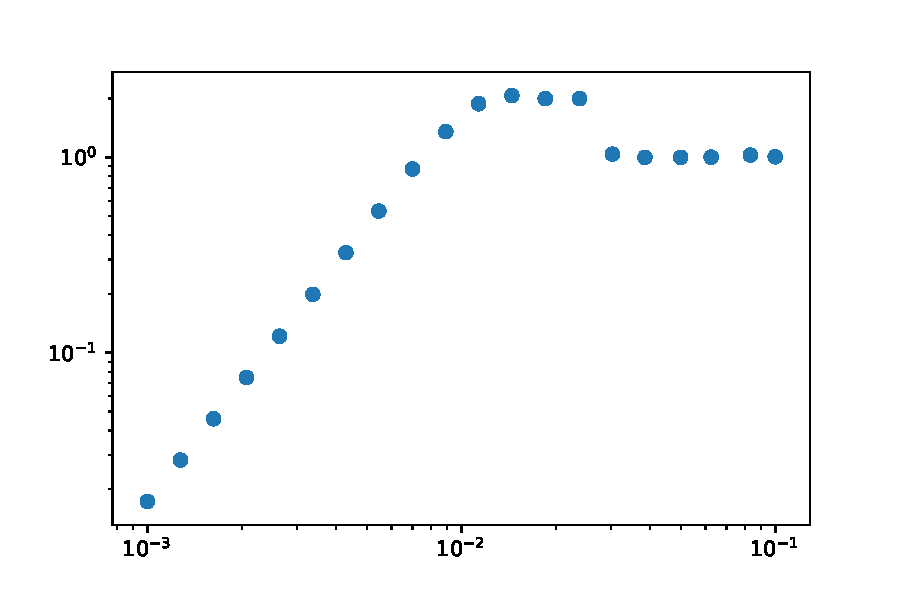
\includegraphics[width=\textwidth]{code/error.pdf}
    \caption{infinity norm of error vs. \( h \)}
\end{subfigure}
\begin{subfigure}{.3\textwidth}
    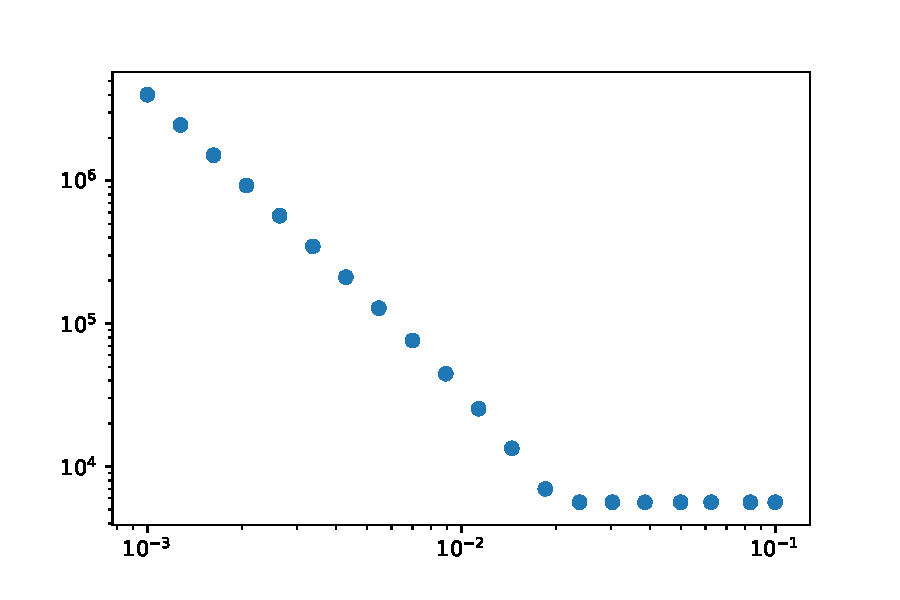
\includegraphics[width=\textwidth]{code/Ah.pdf}
    \caption{\( \norm{A}_\infty \) vs. \( h \)}
\end{subfigure}
\begin{subfigure}{.3\textwidth}
    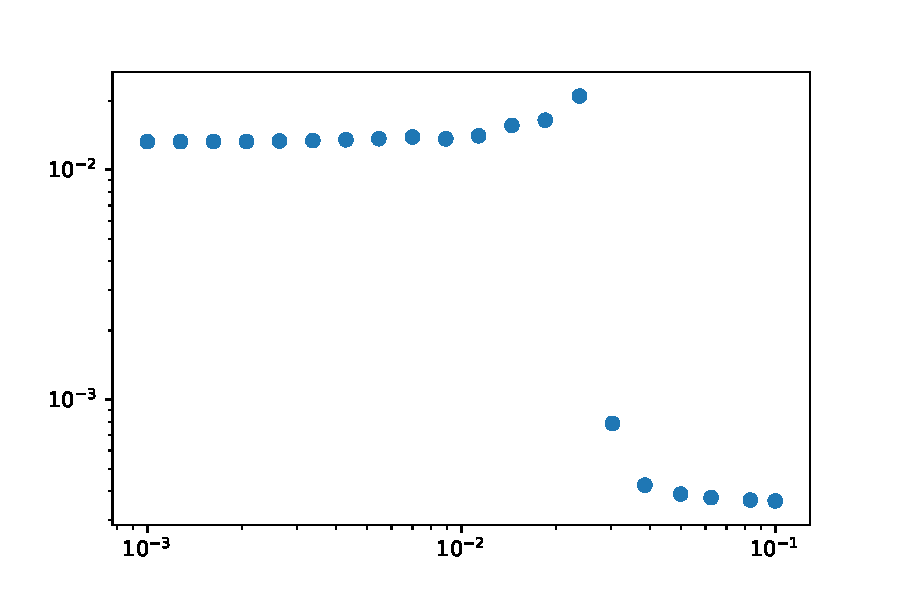
\includegraphics[width=\textwidth]{code/Ahinv.pdf}
    \caption{\( \norm{A^{-1}}_\infty \) vs. \( h \)}
\end{subfigure}
\caption{}
\label{}
\end{figure}


\item Jacobi iteration will converge if and only if \( \rho(I-M^{-1}A) < 1 \), where \( M = \operatorname{diag}(A) \).

We see that the Jacobi iteration does not converge for values of \( h \) above a certain threshold.

The vertical asymtote happens around \( m=53 \approx k/\sqrt{2} \) where the diagonal entries of most of the matrix are zero.

\note{WHY}

\begin{figure}[H]\centering
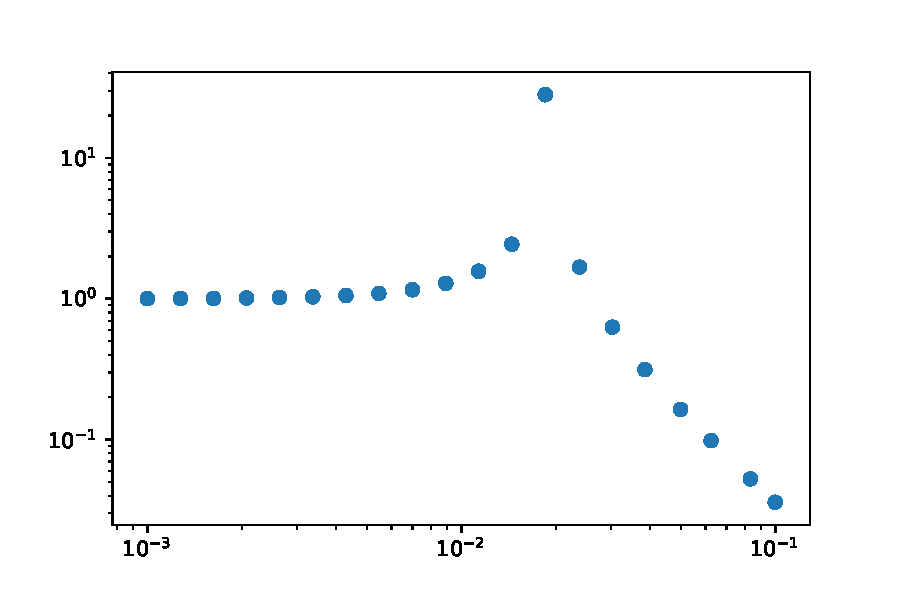
\includegraphics[width=.5\textwidth]{code/spect.pdf}
\caption{spectral radius of \( I-M^{-1}A \) vs. \( h \)}
\end{figure}

\end{itemize}
\end{solution}

\begin{problem}[Winter 2011, Day 2, Problem 5]
Consider the Helmholtz problem,
\begin{align*}
    u_{xx}+u_{yy}+k^2u = f(x,y)=(k^2-5\pi^2)\sin(\pi x)\sin(2\pi y)
\end{align*}
with \( u(x,y) = 0 \) on the boundary of the unit square, \( (x,y) \in [0,1]^2 \).
\begin{enumerate}[label=(\alph*),nolistsep]
    \item Solve the Helmholtz problem using the 5-point Laplacian (second order finite difference) and the backslash as linear system solver. Verify your code works for \( k = 5\), \( k = 10\), and \( k = 60 \) by giving log-log plots for the maximum nodal error as a function of \( h \).
    \item Suppose we change the solver to Jacobi (say take 200 iterations of Jacobi’s method). Program this in your code using the matrix version of Jacobi. Derive the spectral radius of Jacobi’s iteration matrix in terms of \( h \) and \( k \). Recall the eigenvalues \( \lambda_{pq} \) of the 5-point Laplacian are,
    \begin{align*}
        \dfrac{2}{h^2}(\cos(p\pi h)+\cos(q\pi h)-2)
    \end{align*}
    where \( h=1/(m+1) \), \( p=1,2,\ldots, m \), \( q=1,2,\ldots, m \).
    \item If we fix \( h=1/21 \), for what values of \( k \) will Jacobi's method converge? Verify this in your code by trying \( k=5 \), \( k=10 \), and \( k=60 \), and any other \( k \) values, say \( k=0 \) for example, you deem appropriate.
\end{enumerate}
\end{problem}

\begin{solution}[Solution]
\begin{enumerate}[label=(\alph*)]
\item Note that \( u(x) = \sin(\pi x)\sin(2\pi y) \) is the solution to this equation for any \( k \).

\begin{lstlisting}
for k in [5,10,60]:
    def f(x,y):
        return (k**2-5*np.pi**2)*np.sin(np.pi*x)*np.sin(2*np.pi*y)

    def u_true(x,y):
        return np.sin(np.pi*x)*np.sin(2*np.pi*y)

    mesh_sizes = np.array([3,9,30,99,299]);
    max_error = np.zeros(len(mesh_sizes));

    for j,m in enumerate(mesh_sizes): # number of interior mesh points in a given direction
        h = 1/(m+1)


        # construct A
        T = sp.sparse.diags([-4*np.ones(m),np.ones(m-1),np.ones(m-1)],[0,1,-1])

        A = sp.sparse.kron(sp.sparse.eye(m),T) + sp.sparse.kron(sp.sparse.diags([np.ones(m-1),np.ones(m-1)],[-1,1]),sp.sparse.eye(m))

        A /= h**2
        A += k**2 * sp.sparse.eye(m*m)

        # construct right hand side F
        xy = np.linspace(0,1,m+2)[1:-1] # get position of interior points

        F = np.reshape([[f(x,y) for x in xy] for y in xy],-1)

        # solve system
        U = sp.sparse.linalg.spsolve(A,F)

        U_true = np.reshape([[u_true(x,y) for x in xy] for y in xy],-1)

        max_error[j] = np.max(np.abs(U-U_true))


    plt.figure()
    plt.scatter(np.log10(1/(mesh_sizes+1)),np.log10(max_error),color='k')
    plt.savefig('w2011d2p5_'+str(k)+'.pdf')
\end{lstlisting}


\begin{figure}[H]\centering
\foreach \k in {5,10,60} {
\begin{subfigure}{.3\textwidth}\centering
    \includegraphics[width=\textwidth]{code/w2011d2p5_\k.pdf}
    \caption{\(k=\k\)}
\end{subfigure}
}
\caption{max nodal error vs. mesh size}
\label{}
\end{figure}

\item
Recall the Jacobi method is of the form,
\begin{align*}
    x_k = x_{k-1} + M^{-1} (b-Ax_{k-1}) = b+(I-M^{-1}A)x_{k-1}
\end{align*}

Thus,
\begin{align*}
    e_k = (I-M^{-1}A)e_{k-1} = (I-M^{-1}A)e_0
\end{align*}

We implement Jacobi iteration is Numpy as,
\begin{lstlisting}
def jacobi(A,b,x,max_iter):
    M = sp.sparse.diags(A.diagonal())
    for n in range(max_iter):
        r = b-A@x
        x += sp.sparse.linalg.spsolve(M,r)
    return x
\end{lstlisting}

Note that the eigenvalues of \( A \) are,
\begin{align*}
    k^2 + \dfrac{2}{h^2}(\cos(p\pi h)+\cos(q\pi h)-2)
\end{align*}



Now note that \( M = \operatorname{diag}(A) = (k^2 - 4/h^2) I \) so the eigenvalues of \( I - M^{-1}A = I - (k^2 - 4/h^2)^{-1} A \) are,
\begin{align*}
    1 - \left( k^2 - \frac{4}{h^2} \right)^{-1}\left( k^2 + \dfrac{2}{h^2}(\cos(p\pi h)+\cos(q\pi h)-2) \right)
\end{align*}

We can rewrite this as,
\begin{align*}
    \lambda(h,k,p,q) = 1 - \frac{ h^2k^2 + 2(\cos(p\pi h)+\cos(q\pi h)-2)}{h^2k^2 - 4}
\end{align*}

It is clear that fixed \( h \) and \( k \), the above expression is identical when \( p=q=1 \) or \( p=q=m \).

Note that this is a linear function of \( \cos(p\pi h) + \cos(q\pi h) \).
Now take \( p \) away from one of these points. The expression decreases.
Thus,
\begin{align*}
    \rho(I-M^{-1}A) = \left| 1 - \dfrac{h^2k^2 + 2(\cos(\pi h)+\cos(\pi h)-2) }{h^2k^2-4} \right|
\end{align*}


\item
Jacobi iteration will converge if and only if \( \rho(I-M^{-1}A) < 1 \). We require,
\begin{align*}
    -1 < 1 - \dfrac{h^2k^2 + 2(\cos(m\pi h)+\cos(m\pi h)-2) }{h^2k^2-4} < 1
\end{align*}

We solve \( |1 - (h^2k^2-4)^{-1}(h^2k^2 + 2(\cos(m\pi h)+\cos(m\pi h)-2)) |=1 \) with Mathematica and obtain solutions,
\begin{align*}
    k = \pm 42\sqrt{1+\cos(\pi/21)}, \pm 42\sqrt{1-\cos(\pi/21)}
\end{align*}

Using the plot (and assuming \( k>0 \)) it is clear that for any
\begin{align*}
    k &\notin \left(42\sqrt{1-\cos(\pi/21)},42\sqrt{1+\cos(\pi/21)}\right) \approx(4.43874,59.2309)
\end{align*} the method will converge.
This is observed in our tests.

\end{enumerate}
\end{solution}


\begin{problem}[Summer 2013, Day 3, Problem 1]
Consider the PDE,
\begin{align*}
    4u_{xx}+12u_{xy}+9u_{yy} = 0
\end{align*}
on the rectangle \( 0\leq x\leq 2 \), \( 0\leq y\leq 3 \) with boundary conditions,
\begin{align*}
    u(x,0) = 0, && u(x,3)=3, && u(0,y) = 2, && u(2,y)=1
\end{align*}
\begin{enumerate}[nolistsep]
\item Develop a finite difference method for this problem on a uniform grid with \( \Delta x =
\Delta y = h \), and use it to solve the problem. Discuss the order of accuracy and convergence of your method.
\item Find an analytical solution to the problem.
\item Suppose that the coefficient of the cross-term \( u_{xy} \) in the PDE were \( 12-\epsilon \) instead of 12, where \( \epsilon \) is a small positive number. Call the solution to this modified problem \( u_\epsilon(x, y) \). Let \( M(\epsilon) \) be the max-norm of \( |u_\epsilon(xm y) - u(x, y)| \) over the rectangle. Can you estimate how \( M(\epsilon) \) scales with \( \epsilon \)?
\end{enumerate}

\end{problem}


\begin{solution}[Solution]
\begin{enumerate}[]
\item Let \( m = 2/h-1 \) and \( n = 3/h-1 \) be the number of interior points in the \( x \) and \( y \) directions.

For \( i \in (1,m+1)\cap \ZZ \),
\begin{align*}
    u_{xx} \approx \frac{u_{i+1,j}+u_{i-1,j}-2u_{i,j}}{h^2}
\end{align*}

For \( j\in(1,n+1)\cap\ZZ \),
\begin{align*}
    u_{yy} \approx \frac{u_{i,j+1}+u_{i,j-1}-2u_{i,j}}{h^2}
\end{align*}

For \( (i,j)\in(1,m+1)\times(1,n+1)\cap\ZZ^2 \),
\begin{align*}
    u_{xy} \approx \dd{}{x} \frac{u_{j+1}(x) - u_{j-1}(x) }{2h} = \frac{u_{i+1,j+1} + u_{i-1,j-1} - u_{i+1,j-1} - u_{i-1,j+1}}{4h^2}
\end{align*}

For \( i,j \) with \( 1<i<m+1 \) and \( 1<j<m+1 \),
\begin{align*}
    &4\frac{u_{i+1,j}+u_{i-1,j}-2u_{i,j}}{h^2} \\
    & \hspace{6em}+ 12 \frac{u_{i+1,j+1} + u_{i-1,j-1} - u_{i+1,j-1} - u_{i-1,j+1}}{4h^2} \\
    & \hspace{18em}  + 9 \frac{u_{i,j+1}+u_{i,j-1}-2u_{i,j}}{h^2} = 0
\end{align*}

This gives the stencil,
\begin{align*}
\begin{array}{ccc}
-3 & 9 & 3 \\
4 & -26 & 4 \\
3 & 9 & -3 \\
\end{array}
\end{align*}

Using the standard ordering we have matrix equation,
\begin{align*}
    A = \left[\begin{array}{cccc}T & T_1
    \\ T_2 & T & T_1
    \\ & \ddots & \ddots & \ddots
    \end{array}\right]
\end{align*}
where,
\begin{align*}
T = \left[\begin{array}{cccc}
-26 & 4 \\
4 & -26 & 4 \\
& \ddots & \ddots & \ddots
\end{array}\right],&&
T_1 = \left[\begin{array}{cccc}
9 & 3 \\
-3 & 9 & 3 \\
& \ddots & \ddots & \ddots
\end{array}\right],&&
T_2 = T_1^T
\end{align*}

We deal with the boundary conditions by modifying the right hand side.

We implement this in Python,
\begin{lstlisting}
m = 30
n = 50


T = sp.sparse.diags([-26*np.ones(m),4*np.ones(m-1),4*np.ones(m-1)],[0,1,-1])

T1 = sp.sparse.diags([9*np.ones(m),3*np.ones(m-1),-3*np.ones(m-1)],[0,1,-1])

T2 = T1.T

A = sp.sparse.kron(sp.sparse.eye(n,k=0),T)
A += sp.sparse.kron(sp.sparse.eye(n,k=1),T1)
A += sp.sparse.kron(sp.sparse.eye(n,k=-1),T2)

F = np.zeros(m*n)

for j in range(n):
    for i in range(m):
        k = j*m+i
        print((i,j),k)
        if i == 0: #left boundary
            F[k] += 4*2
        if i == m-1: #right boundary
            F[k] += 4*1
        if j == 0: #bottom boundary
            F[k] += 9*0
        if j == n-1: #top boundary
            F[k] += 9*3

U = sp.sparse.linalg.spsolve(A,-F)

u = np.reshape(U,(n,m))
plt.pcolor(u)
plt.axis('image')
\end{lstlisting}


\item \note{no idea, not relevant}

\item \note{no idea, not relevant}

\end{enumerate}
\end{solution}

\begin{problem}[Summer 2014, Day 1, Problem 5]
The Matlab code poisson.m provided to you solves the problem,
\begin{align*}
    u_{xx}+u_{yy}=-5\pi^2\sin(\pi x)\sin(2\pi y)
\end{align*}
with \( u(x, y) = 0 \) on the boundary of the unit square \( 0 \leq x \leq 1 \), \( 0 \leq y \leq 1 \).

The mesh spacing \( h \) is taken the same in both coordinate directions and \( h = 1/(m + 1) \) where there are m interior unknowns in each row and each column. This code uses sparse storage to create a matrix problem \( A^hu^h = F^h \) where the interior unknowns are by rows, bottom to top, and within each row, from left to right using the natural rowwise ordering. The code is set up to solve this problem using \( m = 20 \). It uses Matlab’s backslash command to solve the linear system. The true solution to this PDE is known and used in the code to set the correct boundary conditions. The norm \( \norm{u^h − u_{pde}}_\infty \) measuring the max error in the discrete solution relative to the PDE at the nodal points
is printed at the end.

Recall, the eigenvalues \( \lambda_{pq} \) of \( A^h \) are \( (2/h^2)(\cos(p\pi h)+\cos(q\pi h)-2) \) where \( p = 1, 2, \ldots, m \), \( q = 1, 2, \ldots, m \).

\begin{enumerate}[nolistsep]
\item Modify the poisson.m code to solve the Helmholtz problem,
\begin{align*}
    u_{xx} + u_{yy} + k^2u = (k^2 - 5\pi^2) \sin(\pi x) \sin(2\pi y)
\end{align*}
with \( u(x, y) = 0 \) on the boundary of the unit square \( 0\leq x\leq 1 \), \( 0\leq x\leq 1 \). You will need to know the exact solution to this new PDE to set the boundary conditions using the code’s approach.
\item Solve the new problem using your modified code which still uses backslash as the linear system solver. Verify it works for \( k = 3 \), \( k = 10 \), and \( k = 60 \). Do you think the backslash command did any pivoting for any of these problems?
\end{enumerate}
\end{problem}

\begin{solution}[Solution]
\begin{enumerate}[]
    \item This was done in Winter 2011, Day 2, Problem 5
    \item Probably need pivoting if \( k > \sqrt{2}/\pi \) as the matrix will not longer be SPD in this case.
    
    \note{Check this later}
\end{enumerate}
\end{solution}

\begin{problem}[Summer 2014, Day 3, Problem 3]
A heavily used method for solving \( Ax = b \) where \( A \) is sparse, nonsingular, and nonsymmetric is the Krylov-space method called GMRES. Starting with any initial guess \( x_1 \), the method at step \( k \) chooses \( x_{k+1} = x_k + Qy \) where \( Q \) is an \( n \times k \) matrix with orthonormal columns and \( y \) is a \( k \times 1 \) vector.
\begin{enumerate}[nolistsep]
\item Derive the method by showing how \( Q \) and \( y \) are chosen.
\item Show how the Arnoldi process is used in the method.
\item Discuss the arithmetic complexity and convergence properties. How does the truncated GMRES compare to the untruncated algorithm in both complexity and convergence properties?
\item Program as much of the algorithm as you can by either using pseudo code or actual Matlab code.
\end{enumerate}

\end{problem}

\begin{solution}[Solution]
\begin{enumerate}[]
\item The GMRES algorithm minimizes the 2-norm of the residual over successive Krylov spaces. In particular the columns of \( Q_k \) form an orthonormal basis for the space \( \cK_k= \operatorname{span}\{r_0, Ar_0, \ldots, A^{k} r_0\} \) (where we have used the \( k \) to make the dependence of \( Q \) on \( k \) explicit) and at each step we pick \( y\in\RR^k \) minimizing,
\begin{align*}
    \norm{r_{k+1}} = \norm{b-Ax_{k+1}} = \norm{b-Ax_k-AQ_ky} = \norm{r_0-AQ_ky}
\end{align*}
Once we have found this \( y \), the iterate \( x_{k+1} \) is obtained by \( x_{k+1} =  \).

Note that the \( y \) we have described is not quite the same as the \( y \) listed in the question statement. In particular, since \( x_{k}\in\cK_k \) we can write it as \( Q_{k-1} z \), where the last entry of \( z \) is zero. Therefore the \( y \) in the solution varies from the \( y \)in the problem by this amount.

\note{Indexing might be off by one}

\item The Arnoldi algorithm produces an orthonormal basis for \( \cK_k = \operatorname{span}\{r_0, Ar_0, \ldots A^k r_0\} \). When used in GMRES, this is used to construct \( Q \). In particular, the Arnoldi algorithm start with some \( q_1 = r_0 / \norm{r_0} \) and orthogonalizes \( Aq_1 \) against this vector to produce \( q_2 \). This process is repeated, and can be written
\begin{align*}
    AQ_k = Q_{k+1}H_{k+1,1}
\end{align*}
for an upper Hessenberg matrix \( H \),

Thus, instead of explicitly minimizing \( \norm{r_{k+1}} \) we can instead solve the equivalent system,
\begin{align*}
    \min_{y\in\RR^k} \norm{r_0 - Q_kH_{k+1,k}y} = \min_{y\in\RR^k} \norm{\beta \xi_1 - H_{k+1,k}y}
\end{align*}
where we have used the fact that \( r_0 = \norm{r_0}q_1 = \norm{r_0} Q_k \xi_1 \) and defined \( \beta = \norm{r_0} \).

\item
Unlike conjugate gradient for HPD matrices, GMRES requires that all of \( Q \) be stored.

Similarly to CG, in exact arithmetic GMRES will converge in at most \( n \) iterations. However, due to floating point error, it may be the case that more than \( n \) iterations are required.

One variant of GMRES does not save all of \( Q \), but ocassional resets itself. This saves storage space and reduces the number of operations needed, however it will obviously converge less quickly on some problems.

\item
\begin{itemize}
    \item start with any initial guess \( x_0 \) and compute \( r_0 = b-Ax_0 \). Set \( q_0 = r_0 / \norm{r_0} \).
    \item for \( k=1,2,\ldots \):
    \begin{itemize}
        \item Run one more step of arnoldi to obtain \( Q_{k+1} \) and \( H_{k+1,k} \) satisfying, \( AQ_k = H_{k+1,k}Q_{k+1} \)
        \item compute \( x = r_0 + Q_ky_k \) where \( y_k \) minimizes \( \norm{\beta \xi_1 - H_{k+1,k} y} \)
    \end{itemize}
\end{itemize}

Note that a QR decomposition of \( H_{k+1,k} \) can be used at each step and can be saved and updated rather than recomputed.

\end{enumerate}
\end{solution}


\begin{problem}[Summer 2010, Day 1, Problem 4]
Consider the two-step Adams-Bashforth method to solve the scalar equation \( y' = f(t,y) \):
\begin{align*}
    y_{n+2} = y_{n+1} + h \left[ \frac{3}{2} f(t_{n+1},y_{n+1})-\frac{1}{2} f(t_n,y_n) \right]
\end{align*}
Show that this method is convergent, find its order, and sketch its region of absolute stability. In particular, determine where this region intersects the real and imaginary axes.
\end{problem}

\begin{solution}[Solution]
This is a linear multistep method of the form,
\begin{align*}
    \sum_{j=0}^{r} \alpha_{j} U^{n+1} = h\sum_{j=0}^{r} \beta_j f(U^{n+j},t_{n+j})
\end{align*}
where \( r = 2 \), \( \alpha_0 = 0 \), \( \alpha_1 = -1 \), \( \alpha_2 = 1 \), \( \beta_0 = -1/2 \), \( \beta_1 = 3/2 \), and \( \beta_2 = 0 \).

The local truncation error is given by,
\begin{align*}
    \tau_n = \frac{y(t_{n+2}) - y(t_{n+1})}{h} - \frac{3}{2} y'(t_{n+1}) + \frac{1}{2} y' (t_n)
\end{align*}

We expand,
\begin{align*}
    y(t_{n+2}) = y(t_{n+1}) + h y'(t_{n+1}) + \frac{h^2}{2} y''(t_{n+1}) + \frac{h^3}{3!} y'''(t_{n+1}) + \cO(h^4)
\end{align*}

Thus,
\begin{align*}
    \frac{y(t_{n+2})-y(t_{n+1})}{h} = y'(t_{n+1}) + \frac{h}{2} y''(t_{n+1}) + \frac{h^2}{3!} y'''(t_{n+1}) +\cO(h^3)
\end{align*}

Now expand,
\begin{align*}
    y'(t_{n}) = y'(t_{n+1}) - h y''(t_{n+1}) + \frac{h^2}{2} y'''(t_{n+1}) + \cO(h^3)
\end{align*}

Finally we see that,
\begin{align*}
    \tau_n &= y'(t_{n+1}) + \frac{h}{2} y''(t_{n+1}) + \frac{h^2}{3!} y'''(t_{n+1}) + \cO(h^3) - \frac{3}{2} y'(t_{n+1}) \\
    &\hspace{5em} + \frac{1}{2} \left[ y'(t_{n+1})-h y''(t_{n+1}) + \frac{h^2}{2!}y'''(t_{n+1}) +\cO(h^3) \right] \\
    &= \frac{5}{12} y'''(t_{n+1}) h^2 + \cO(h^3)
\end{align*}

Therefore the method is consistent and has order \( h^2 \).

The region of absolute stability is the region,
\begin{align*}
    \{ z : \rho(\zeta) - z\sigma(\zeta) \text{ satisfies the root condition} \}
\end{align*}
    where the root condition is that all roots have modulus at most one, and a root with modulus one is simple, and \( \rho(\zeta) = \sum_{j=0}^{r} \alpha_j\zeta^k \) and \( \sigma(\zeta) = \sum_{j=0}^{r} \beta_j \zeta^j \).

In this case we have,
\begin{align*}
    \rho(\zeta) - z\sigma(\zeta) = \zeta^2 - \zeta - z(3/2\zeta - 1/2) = \zeta^2 - (1+3z/2)\zeta + z/2
\end{align*}

Points on the boundary of the region of absolute stability have the form,
\begin{align*}
    z = \rho(e^{i t})/\sigma(e^{it}), && t\in[0,2\pi)
\end{align*}

This looks like an egg to the left of the imaginary axis.

The points on the real axis are \( -1,0 \) and the point on the imaginary axis is \( 0 \).

    \note{double check this and solve analytically?}

\iffalse
The roots of \( \rho(\zeta) - z\sigma(\zeta) \) are,
\begin{align*}
    \zeta = \frac{(1+3z/2) \pm \sqrt{(1+3z/2)^2-2z}}{2}
\end{align*}

We plot the region where both roots are less than or equal to one in modulus using Mathematica. It looks like an egg. 

\note{There is some weird stuff with the branch cut}

To see this analytitcally we set \( \zeta = e^{I t} \) and find,
\begin{align*}
    z = \frac{2}{3} (e^{i t} - e^{-it}) = \cos(t) + i\frac{1}{3}\sin(t) - \frac{2}{3}
\end{align*}

This gives all points on the boundary, and possibly more. However we see that this region is exactly the elipse we expected. The imaginary part is zero when \( \sin(t) = 0 \), and the real part is zero when \( \cos(t) = 2/3 \). By setting \( t=\arcsin(0) \) and \( t=\arcsin(2/3) \) we have intersection points,
\begin{align*}
    -2/3 \pm 1,  &&  \pm  i \frac{\sqrt{5}}{9}
\end{align*}

\fi

Since the origin is contained in the region of absolute stability, the method is zero-stable. Since it is also consistent the method is convergent.

\end{solution}




\begin{problem}[Winter 2010, Day 1, Problem 3]
Consider the one-step Adams-Moulton method (also known as the trapezoidal rule) to
solve the scalar equation \( y_0 = f(t, y) \):
\begin{align*}
    y_{n+1} = y_n + \frac{h}{2} \left[ f(t_{n+1},y_{n+1}) + f(t_n,y_n) \right]
\end{align*}
\begin{itemize}[nolistsep]
\item Is this an explicit or an implicit method? Why?
\item Show that this method is convergent, find its order, and sketch its region of absolute stability.
\end{itemize}
\end{problem}

\begin{solution}[Solution]
\begin{itemize}
\item This is an implicit method since we cannot solve for \( y_{n+1} \) without knowing the inverse of \( f \).
\item This is a linear multistep method of the form,
    \begin{align*}
        \sum_{j=0}^{r} \alpha_{j} U^{n+1} = h\sum_{j=0}^{r} \beta_j f(U^{n+j},t_{n+j})
    \end{align*}
        where \( r = 1 \), \( \alpha_0 = -1 \), \( \alpha_1 = 1 \), \( \beta_0 = 1/2 \), and \( \beta_1 = 1/2 \).

We have local truncation error,
\begin{align*}
    \tau_n = \frac{y(t_{n+1}) - y(t_n)}{h} - \frac{1}{2} \left[ y'(t_{n+1}) + y'(t_n) \right]
\end{align*}

We expand,
\begin{align*}
    y(t_{n+1}) &= y(t_n) + h y'(t_n) + \frac{h^2}{2} y''(t_n) + \frac{h^3}{3!} y'''(t_n) + \cO(h^4) \\
    y'(t_{n+1}) &= y'(t_n) + h y''(t_n) + \frac{h^2}{2} y'''(t_n) + \cO(h^3) \\
\end{align*}

Thus,
\begin{align*}
    \tau_n &= y'(t_n) + \frac{h}{2} y''(t_n) + \frac{h^2}{3!}y'''(t_n) + \cO(h^3) - \frac{1}{2} \left[ 2y'(t_n) + hy''(t_n) + \frac{h^2}{2} y'''(t_n) + \cO(h^3) \right] \\
    &= -\frac{1}{3} y'''(t_n) h^2 + \cO(h^3)
\end{align*}

Therefore the method is consistent as \( h\to 0 \), and is order \( h^2 \).

The region of absolute stability is the region,
\begin{align*}
    \{ z : \rho(\zeta) - z\sigma(\zeta) \text{ satisfies the root condition} \}
\end{align*}
    where the root condition is that all roots have modulus at most one, and a root with modulus one is simple, and \( \rho(\zeta) = \sum_{j=0}^{r} \alpha_j\zeta^k \) and \( \sigma(\zeta) = \sum_{j=0}^{r} \beta_j \zeta^j \).

In this case we have,
\begin{align*}
    \rho(\zeta) - z\sigma(\zeta) =  \zeta -1 - z(\zeta/2+1/2) = (1+z/2)\zeta + z/2-1
\end{align*}

The roots of \( \rho(\zeta) - z\sigma(\zeta) \) are,
\begin{align*}
    \zeta = ( z/2-1 ) / (z/2+1)
\end{align*}

We plot the region where this roott is less than or equal to one in modulus using Mathematica.

This gives the entire left half plane (as expected). Since the origin is contained in the region of absolute stability, the method is zero stable. This along with consistency implies convergence.

\end{itemize}
\end{solution}


\begin{problem}[Summer 2011, Day 2, Problem 6]
Consider the following linear multistep method:
\begin{align*}
    y_{n+3} + (2b-3)(y_{n+2}-y_{n+1}) - y_n = hb(f_{n+2}+f_{n+1})
\end{align*}
to approximate the ordinary differential equation
\begin{align*}
    \dd{y}{x}(x) = f(x,y(x)), && y(0) = y_0
\end{align*}
(where \( f \) is a smooth function).

\begin{enumerate}[label=(\alph*),nolistsep]
\item Determine all values of the real parameter \( b, b \neq 0\), for which the
method is zero-stable.
\item Show that the truncation error,
\begin{align*}
    T_n = \frac{y(x_{n+3})+(2b-3)(y(x_{n+2})-y(x_{n+1}))-y(x_n)-hb(f(x_{n+2})+f(x_{n+1}))}{2hb}
\end{align*}
(where \( y \) is a solution to the ordinary differential equation) is \( \cO(h^2) \) when the method is zero-stable.
\item Show that there exists a value of \( b \) for which the truncation error is \( \cO(h^4) \).
\end{enumerate}
\end{problem}

\begin{solution}[Solution]
\begin{enumerate}[label=(\alph*)]
    \item This is a linear multistep method with characteristic polynomial,
        \begin{align*}
            \rho(\zeta) &= \zeta^3 + (2b-3)\zeta^2 - (2b-3)\zeta - 1 
            \\&= (\zeta - 1)(\zeta - 1 +b + \sqrt{b^2-2b})(\zeta-1+b-\sqrt{b^2-2b})
        \end{align*}

        The roots are then,
        \begin{align*}
            1, && 1-b \pm \sqrt{b^2-2b}
        \end{align*}
        
        The method is zero stable if all roots have modulus less than or equal to one, and any roots of modulus one are simple. 
        
        First observe \( b^2-2b \geq 0 \) when \( b\leq 0 \) or \( b\geq 2 \) so the roots have size larger than one and do not satisfy the root condition.

        Now observe that for \( b=1 \) and \( b=0 \) the roots are repeated and do not satisfy the root condition.

        Suppose \( b\in(0,2) \). Then \( |\zeta|^2 = (1-b)^2 + i^2 ((b-1)^2-1) =1 \). And the roots are different so the root condition is satisfied.



        \iffalse
        When the method is zero-stable we have truncation error,
       \begin{align*}
           T_n = \frac{y(x_{n+3})+y(x_{n+2})-y(x_{n+1})-y(x_n)-2h(f(x_{n+2})+f(x_{n+1}))}{4h}
       \end{align*}
    
        We rewrite this as,
        \begin{align*}
            T_n &= \frac{1}{2} \left[ \frac{y(x_{n+3})-y(x_{n+1})}{2h} + \frac{y(x_{n+2})-y(x_n)}{2h} \right] - \frac{1}{2} \left[ y'(x_{n+2})+y'(x_{n+1}) \right] \\
            &= \frac{1}{2} \left[ y'(x_{n+2}) + \cO(h^2) + y'(x_{n+1}) + \cO(h^2) \right] - \frac{1}{2} \left[ y'(x_{n+2}) + y'(x_{n+1}) \right]
            &= \cO(h^2)
        \end{align*}
        
        Note that while we have proved that the truncation error is \( \cO(h^2) \) as instructed, it is possible that it is actually higher order (although I don't think that this is the case).
        \fi
    \item
        We do this in Mathematica because fuck Taylor expansions.

        First define,
        \begin{lstlisting}
            S[j_] := Series[f[x + j h], {h, 0, 5}]
        \end{lstlisting}
        
        This will compute the Taylor exapnsion of \( f(x+j h) \) up to 5-th order.

        Now compute the truncation error and simplify,
        \begin{lstlisting}
            FullSimplify[(S[3] + (2 b - 3) (S[2] - S[1]) - S[0])/(2 h b) - (D[f[x + 2 h], x] + D[f[x + h], x])/2]
        \end{lstlisting}

        This shows the truncation error is order \( h^2 \).

    \item 
        From this the output of this it is clear that choosing \( b=6 \) gives the desired order of accuracy.

        In particular we have truncation error,
        \begin{align*}
            T_n = \frac{1}{120}f^{(5)}(x)h^4 + \cO(h^5)
        \end{align*}       

\end{enumerate}
\end{solution}


\begin{problem}[Summer 2012, Day 2, Problem 3]
Consider the scheme
\begin{align*}
    u_{n+1} = u_n + hf(t_n+(1-\theta)h,\theta u_n+(1-\theta)u_{n+1})
\end{align*}
for solving the ODE \( u' = f(t,u) \). Here \( u_n \) and \( u_{n+1} \) are meant to approximate \( u(t_n) \) and \( u(t_{n+1}) = u(t_n+h) \), respectively.
\begin{enumerate}[label=(\alph*),nolistsep]
    \item For all \( \theta \in [0,1] \), find the order of this scheme.
    \item Determine for which \( \theta\in[0,1] \) the scheme is convergent.
    \item For \( \theta_0 = 0 \) and \( \theta_1 = 1 \) determine the stability domain of the scheme.
    \item Consider the system,
    \begin{align*}
        \dd{}{t} \left[\begin{array}{c}u_1 \\ u_2\end{array}\right]
        =
        \left[\begin{array}{cc}-a & 0 \\ 0 & -1/a\end{array}\right]
        \left[\begin{array}{c}u_1 \\ u_2\end{array}\right]
        + \frac{\pi}{a} \left[\begin{array}{c}u_1u_2 \\ u_2^2 - u_1 \end{array}\right]
    \end{align*}
    where \( a \) is a positive parameter. Find its equilibrium points and determine their linear stability. Are your results qualitatively the same for all values of \( a > 0 \)? For \( a = 10 \), draw a phase portrait that is qualitatively consistent with your findings. This plot does not have to be to scale.
    \item Choose a suitable value of \( \theta \) and using the scheme above, produce a plot of the curve \( [u_1(t), u_2(t)]^T \) with initial conditions \( [1,-1]^T \) in the phase plane. Run the scheme until you get ``reasonably'' close to an equilibrium point.
\end{enumerate}
\end{problem}

\begin{solution}[Solution]
\begin{enumerate}[label=(\alph*)]
    \item
        We have truncation error,
        \begin{align*}
            \tau_n = \frac{u(t_{n+1}) - u(t_n)}{h} - f(t_n + (1-\theta) h, \theta u(t_n) + (1-\theta)u(t_{n+1}))
        \end{align*}

        Write,
        \begin{align*}
            f(t_{n+1} - \theta h, u(t_{n+1}) - \theta(\Delta u))
        \end{align*}
        

        Write \( t = t_n \), \( u = u(t_n) \), \( \Delta t = (1-\theta) h \), and \( \Delta u = (1-\theta) (u(t_{n+1}) - u(t_n)) \). 
        Observe,
        \begin{align*}
            \Delta u &= (1-\theta)(u(t_{n+1}) - u(t_n)) \\
            &= (1-\theta)\left( h u'(t_n) + \frac{h^2}{2} u''(t_n) + \cO(h^3) \right) \\
            &= \Delta t u'(t_n) + (1-\theta)\left( \frac{h^2}{2} u''(t_n) + \cO(h^3) \right)
        \end{align*}
        
        Therefore,
        \begin{align*}
            \cO(\Delta t)  = \cO(\Delta u) = \cO(h) 
        \end{align*}

        Expand and simplify using \( u'' = f_t(t,u) + f_u(t,u)u'(t) \),
        \begin{align*}
            f(t + \Delta t, u + \Delta u)
            &= f(t,u) + \Delta t f_t(t,u) + \Delta u f_u(t,u) + \cO(\Delta t^2 + \Delta t\Delta u + \Delta u^2) 
            \\&= f(t,u) + \Delta t \left (f_t(t,u) + u'(t) f_u(t,u) \right) + \cO(h^2) 
            \\&= u'(t) + \Delta t u''(t)  + \cO(h^2) 
        \end{align*}

        Thus,
        \begin{align*}
            \tau_n = \frac{h}{2}u''(t_n) - (1-\theta) h u''(t_n) + \cO(h^2)
        \end{align*}
        
        Therefore the scheme has local truncation error \( \cO(h) \), and when \( \theta = 1/2 \) it is also \( \cO(h^2) \).

        While we have not proved that when \( \theta=1/2 \) the scheme is not actually higher order, we guess that it is very unlikely that this is the case.

    \item 
        \note{Flesh this argument out}

        \note{easier to prove general case}

        We have,
        \begin{align*}
            u(t_{n+1}) = u(t_n) + h f(t_n+(1-\theta)h, \theta u(t_n) + (1-\theta)u(t_{n+1})) + \tau
        \end{align*}
        

        \begin{align*}
            d_{n+1} &= u(t_{n+1})-u_{n+1}
            \\&= d_n + h [ 
            f(t_n+(1-\theta)h,\theta u(t_n)+(1-\theta)u(t_{n+1}))
            \\&\hspace{5em}-f(t_n+(1-\theta)h,\theta u_n+(1-\theta)u_{n+1})
            ]
        \end{align*}
        

        \begin{align*}
            |d_{n+1}| \leq |d_n| + h L(\theta |d_n| + (1-\theta)|d_{n+1}|) + h\tau
        \end{align*}
        

        \begin{align*}
            |d_{n+1}|(1-hL(1-\theta)) \leq |d_n|(1+hL\theta) + h\tau
        \end{align*}
        
        Assume \( h \) small enough so that \( 1-hL(1-\theta) \geq 1/2 \). Then,
        \begin{align*}
            |d_{n+1}| &\leq \frac{1+hL\theta}{1-hL(1-\theta)}|d_n| + \frac{1}{1-hL(1-\theta)} h \tau
            \\&:= r|d_n| + s h \tau
            \\ &\leq r^{n+1}|d_0| + s h \tau \left( \sum_{j=0}^{n} r^j \right)
            \\ &= r^{n+1}|d_0| + sh \tau \left( \frac{r^{n+1}-1}{r-1} \right)
        \end{align*}
        
        \begin{align*}
            r = \frac{1+hL\theta - hL + hL}{1+hL\theta - hL}
            = 1 + \frac{hL}{1+hL\theta - hL}
        \end{align*}
        
        Then,
        \begin{align*}
            r^{n+1} \leq e^{(n+1) hL/(1+hL\theta-hL)} \leq e^{TL/(1+hL\theta - hL)} \leq e^{2TL}
        \end{align*}
        
        Therefore \( r^{n+1} \) is bounded as \( h\to 0 \).
        
        Note that,
        \begin{align*}
            \frac{sh}{r-1} = \frac{sh}{hLs} = \frac{1}{L}
        \end{align*}
        
        This means \( hs(r^{n+1}-1)/(r-1) \) is bounded, so since \( \tau \to 0 \) the method is convergent.

        Therefore for any \( \theta \) the method is convergent.


   \item When \( \theta = 0 \) this is backward Euler and has stability region outside of the circle of radius 1 centered at 1. Similarly, when \( \theta = 1 \) this is forward Euler and has stability region inside the circle of radius 1 centered at \( -1 \).
    
    \note{stability domain == region of absolute stability??} 

    \item \note{Not relevant}
    \item \note{do this later??} 
\end{enumerate} 
\end{solution}


\begin{problem}[Winter 2015, Day 1, Problem 3]
Consider the linear multistep method,
\begin{align*}
    U^{n+2} = U^{n+1} + \frac{k}{2}(3 f(U^{n+1}) - f(U^n)),
\end{align*}
as a method for solving the ODE initial value problem \( u_0(t) = f(u(t)) \) with step size \( k \).
\begin{enumerate}[label=(\alph*),nolistsep]
\item Is the method \textit{convergent}? Explain what this term means and justify your answer.
\item Determine the order of accuracy and the leading term in the local truncation error.
\item Does the point \( z = -1 \) lie in the region of absolute stability for this method? Justify your answer.
\end{enumerate}
\end{problem}

\begin{solution}[Solution]
\begin{enumerate}[label=(\alph*)]
\item Convergent means that the numerical solution at a given value of \( t \) converges to the actual solution at this value of \( t \) in the limit as \( k\to 0 \). This is a linear multistep method so we have convergence if and only if we have stability and consistency.

    \note{Can I determine this without LTE?}

    The method is consistent as shown in (b). Since \( \rho(\zeta) = \zeta^2 - \zeta \) has roots of, \( \zeta = 0 \), and \( \zeta = 1 \) the method is zero-stable (these roots both have modulus less than or equal to one, and the root of modulus one is simple).

    This means the method is convergent.


\item
    We have local truncation error,
    \begin{align*}
        \tau_n = \frac{u(t_{n+2}) - u(t_{n+1})}{h} - \frac{3u'(t_{n+1}) - u'(t_n)}{2}
    \end{align*}

    Using Mathematica we find,
    \begin{align*}
        \tau_n = \frac{5}{12}u'''(t_n) h^2 + \cO(h^3)
    \end{align*}
    

\item 
    Consider the polynomial,
    \begin{align*}
        \pi(\zeta) = \rho(\zeta) + \sigma(\zeta) = \zeta^2 - \zeta + 3\zeta/2-1/2 = \zeta^2 -\zeta/2 - 1/2 = (\zeta+1/2)(\zeta-1)
    \end{align*}
    The roots are then \( \zeta = -1/2 \) and \( \zeta =1 \). These both have modulus less than or equal to one, and the root with modulus one is simple. Therefore \( z=-1 \) lies in the region of absolute stability.

\end{enumerate}
 
\end{solution}


\begin{problem}[Winter 2017, Day 1, Problem 2]
Consider difference equations of the form,
\begin{align*}
    u_{n+2} + a_1 u_{n+1}+a_0 u_n = kbf(u_{n+1})
\end{align*}
for the initial value problem \( u'(t) = f(u(t)) \), where \( k = t_{n+1} - t_n \) is the timestep.

\begin{enumerate}[label=(\alph*),nolistsep]
    \item Determine the coefficients \( a_0, a_1 \), and \( b \) that give the highest order local truncation error and say what that order is.
    \item Is the resulting method convergnet? Say why or why not.
    \item Determine which, if any, of the points \( -1,\pm i, \pm\frac{1}{2} i \) line in the region of absolute stability.
\end{enumerate}
\end{problem}

\begin{solution}[Solution]
\begin{enumerate}
    \item
    We have local truncation error,
    \begin{align*}
        \tau_n &= \frac{u(t_{n+2}) + a_1 u(t_{n+1}) + a_2 u(t_n)}{k} - b u'(t_{n+1})
        \\&= \frac{1+a_0+a_1}{h} f(t_n) + (2+a_1-b) f'(t_n) + \frac{1}{2} (4+a_1-2b) f''(t_n) h + \frac{1}{6}(8+a_1-3b) + \cO(h^3)
    \end{align*}
    
    We can eliminate the first three terms by choosing, \( a_0 = -1 \), \( a_1 = 0 \), and \( b = 2 \).

    \item Observe,
        \begin{align*}
            \rho(\zeta) = \zeta^2- 1 = (\zeta +1)(\zeta-1)
        \end{align*}
        Therefore the roots are \( \zeta = \pm 1 \), each with modulus less than one and simple. Therefore the method is zero-stable.

        For linear multistep methods we have consistent + zero-stable if and only if convergent.

    \item We have stability polynomial,
        \begin{align*}
            \pi(\zeta;z) = \rho(\zeta) - z\sigma(\zeta) = \zeta^2-1 - z(2\zeta) = \zeta^2 - 2z\zeta -1
        \end{align*}
        This has roots,
        \begin{align*}
            \zeta = z \pm \sqrt{z^2+1}
        \end{align*}
        
        When \( z = -1 \), \( -1-\sqrt{(-1)^2+1} = -1-\sqrt{2} < -1 \) so the root condition is not satisfied.

        When \( z = \pm i \), \( \pm i \pm\sqrt{(\pm i)^2+1} = \pm i \). However in both cases these are repeated roots so the root condition is not satisfied.

        When \( z = \pm i/2 \), \( \pm i/2 \pm \sqrt{(\pm i/2)^2 +1} = \pm i/2 \pm \sqrt{3/4} \). These both have modulus one and are simple so the root condition is satisfied.
\end{enumerate}    
\end{solution}


\begin{problem}[Winter 2010, Day 2, Problem 1]
    Consider the advection equation \( u_t(x,t) + au_x(x,t) = 0 \) defined for all \( x \) where \( a\neq 0 \) is a constant.
    \begin{enumerate}[label=(\alph*),nolistsep]
        \item What is the solution \( u(x,t) \) for \( t > 0 \) if this equation is solved with initial data \( u(x,0) = \eta(x) \)?
        \item Discretize in space with fixed mesh width \( \Delta x \) and time step \( \Delta t \). Explain why the method,
            \begin{align*}
                U_j^{n+1} = U_j^n - \frac{a\Delta t}{2\Delta x}(U_{j+1}^n - U_{j-1}^n)
            \end{align*}
            will not converge to the true solution if we refine in space and time with any fixed ratio \( \Delta t / \Delta x \).
        \item Under what conditions will the method,
            \begin{align*}
                U_j^{n+1} = U_j^n - \frac{a\Delta t}{\Delta x} (U_{j+1}^n-U_j^n)
            \end{align*}
        converge as we refine the grid with fixed ratio \( \Delta t / \Delta x \)?
    \end{enumerate}
\end{problem}

\begin{solution}[Solution]
\begin{enumerate}[label=(\alph*)]
    \item The exact solution is \( u(x,t) = \eta(x-at) \).
    %\item This is forward Euler applied to \( U' = AU \) where \( A \) has \( -a/2h \) on the first super-diagonal, and \( a/2h \) on the first sub-diagonal. This matrix is skew-Hermetian and therefore has purely imaginary eigenvalues. Therefore these eigenvalues are not in the region of absolute stability of forward Euler.
    \item Write \( h = \Delta x \) and \( k = \Delta t \). We replace \( U_j^n \) by \( g(\xi)^n e^{i\xi j h} \) to obtain,
        \begin{align*}
            g(\xi)^n e^{i\xi j h} = g(\xi)^n e^{i\xi j h} - \frac{ak}{h} \left( g(\xi)^n e^{i\xi(j+1)h} - g(\xi)^n e^{i\xi (j-1) h} \right)
        \end{align*}
        Dividing by \( g(\xi)^n e^{i\xi j h} \) we find,
        \begin{align*}
            g(\xi) 
            = 1 - \frac{ak}{2h} \left(e^{i\xi h}-e^{-i\xi h}\right)
            = 1 - i \frac{ak}{h} \sin(\xi h)
        \end{align*}

        Note that the sine can be like \( - 1 + \cO( h ) \) for some values of \( \xi \). In this case, assuming that \( k/h \) is fixed, we have,
        \begin{align*}
            |g(\xi)| = \left|1 + i \frac{ak}{h} + \cO(k)\right| \geq 1 + \cO(k)
        \end{align*}
        
        This proves the method is not convergent.


    \item Write \( h = \Delta x \) and \( k = \Delta t \). We replace \( U_j^n \) by \( g(\xi)^n e^{i\xi j h} \) to obtain,
        \begin{align*}
            g(\xi)^n e^{i\xi j h} = g(\xi)^n e^{i\xi j h} - \frac{ak}{h} \left( g(\xi)^n e^{i\xi(j+1)h} - g(\xi)^n e^{i\xi j h} \right)
        \end{align*}
        Dividing by \( g(\xi)^n e^{i\xi j h} \) we find,
        \begin{align*}
            g(\xi) 
            = 1 - \frac{ak}{h} \left(e^{i\xi h}-1\right)
        \end{align*}

        Note that the \( g(\xi) \) are centered on a circle of radius \( ak/h \) centered at \( 1+ak/h \).

        Thus it is stable whenever \( -1 \leq ah/h \leq 0 \).

        \note{WHAT ABOUT PLUS \( \cO(k) \)??}


\end{enumerate}
\end{solution}


\begin{problem}[Summer 2013, Day 1, Problem 2]
Consider the advection equation \( u_t + au_x = 0 \) and the ``skewed'' upwind method,
\begin{align*}
    U_j^{n+1} = U_{j-1}^n - \left( \frac{a\Delta t}{\Delta x}-1 \right)(U_{j-1}^n - U_{j-2}^n).
\end{align*}
\begin{enumerate}[label=(\alph*),nolistsep]
    \item Show that this method is first order accurate in space and time by computing the local truncation error.
    \item What restriction must be put on the time step \( \Delta t \) in terms of \( \Delta x \) in order for the CFL condition to be satisfied in the case \( a>0 \)? In the case \( a<0 \)?
    \item Show that the method is in fact stable provided the CFL condition is satisfied, i.e., with the bounds found in part (b).
\end{enumerate}
\end{problem}

\begin{solution}[Solution]
\begin{enumerate}[label=(\alph*)]
    \item We have local truncation error,
    \begin{align*}
        \tau = \frac{u(x_j,t_{n+1})-2u(x_{j-1},t_n)+u(x_{j-2},t_n)}{k} + a \left( \frac{u(x_n,t_{j-1})-u(x_n,t_{j-2})}{h} \right)
    \end{align*}
        
    In Mathematica we define,
    \begin{lstlisting}
        U[j_, n_] := Series[Series[u[x + j h, t + n k], {k, 0, 2}], {h, 0, 2}]
    \end{lstlisting}
    
    We compute the LTE using,
    \begin{lstlisting}
        FullSimplify[(U[0, 1] - 2 U[-1, 0] + U[-2, 0])/k +  a ((U[-1, 0] - U[-2, 0])/h), Assumptions -> {D[u[x, t], t] + a D[u[x, t], x] == 0}]
    \end{lstlisting}
    
    This shows that,
    \begin{align*}
        \tau_n = \frac{1}{2} u_{tt} k - \frac{3}{2} a u_{xx} h + \frac{1}{k} u_{xx} + \cO(k^2 + h^2)
    \end{align*}

    This proves that the method is first order accurate in space and time. 

    \item Write \(  h = \Delta x \) and \( k = \Delta t \). The stencil depends only on the value of \( U^n \) at \( x_{j-1} \) and \( x_{j-2} \). We therefore require \( -2h < -ak < -h \). Equivalently, \( ak/h \in [1,2] \).


        Thus we need \( a>0 \) and then pick \( k \in[h/a, 2h/a] \).

    \item Write \(  h = \Delta x \) and \( k = \Delta t \). We replace \( U_j^n \) by \( g(\xi)^n e^{i\xi j h} \) to obtain,
        \begin{align*}
            g(\xi)^{n+1} e^{i\xi j h} = g(\xi)^n e^{i\xi(j-1)h} - \left( \frac{a k}{h}-1 \right) \left( g(\xi)^n e^{i\xi (j-1) h} - g(\xi)^n e^{i\xi (j-2) h} \right)
        \end{align*}
        
        Dividing by \( g(\xi)^n e^{i\xi j h} \) we obtain,
        \begin{align*}
            g(\xi) = e^{i\xi h} \left( 1 - \left( \frac{ak}{h}-1 \right) \left( 1-e^{-i\xi h} \right) \right)
        \end{align*}

        The part above in the parenthesis is a circle of radius \( |ak/h-1| \) centered at \( 2-ak/h \). For \( ak/h \in[1,2] \) the circle will be contained in the unit circle centered at the origin. Therefore \( |g(\xi)| \leq 1 \) whenever the CFL condition is satisfied.
        
\end{enumerate}
\end{solution}


\begin{problem}[Summer 2014, Day 2, Problem 1]
Consider the advection equation \( u_t + au_x = 0 \) with periodic bounday conditions.
\begin{enumerate}[label=(\alph*), nolistsep]
    \item Derive the Lax-Wendroff method below where \( U_j^n \approx u(x_j,t_n) \) with \( \Delta t = k \), and \( \Delta x = h \):
        \begin{align*}
            U_j^{n+1} = U_j^n - \frac{ak}{2h} (U_{j+1}^n - U_{j-1}^n) + \frac{a^2k^2}{2h^2} (U_{j-1}^n - 2U_j^n + U_{j+1}^n).
        \end{align*}
    \item What is the order of the method?
    \item Derive the stability condition.
    \item If you program this method, would you expect to see dissipative behavior? Dispersive behavior? Justify your answer by finding a modified PDE on which the method is 3rd order accurate.
\end{enumerate}
\end{problem}

\begin{solution}[Solution]
\begin{enumerate}[label=(\alph*)]
    \item We will derive this by interpolating where the characteristic passing through \( (x_j,t_{n+1}) \) intersects \( t=t_n \) using the value of \( u \) at  \( x_{j-1} \), \( x_j \), and \( x_{j+1} \).

    This is trivially done in Mathematica by,
    \begin{lstlisting}
    Expand[InterpolatingPolynomial[{{x - h, Subscript[u, j - 1]}, {x, Subscript[u, j]}, {x + h, Subscript[u, j + 1]}}, z] /. {z -> x - a k}] 
    \end{lstlisting}
 
    \item 
    Define,
    \begin{lstlisting}
        U[j_, n_] := Series[Series[u[x + j h, t + n k], {k, 0, 4}], {h, 0, 4}]
    \end{lstlisting}
    
    Now compute,
    \begin{lstlisting}
        FullSimplify[ U[0, 1] - (U[0, 0] - (a k)/(2 h) (U[1, 0] - U[-1, 0]) + (a^2 k^2)/(2 h^2) (U[-1, 0] - 2 U[0, 0] + U[1, 0])), Assumptions -> {D[u[x, t], t] + a D[u[x, t], x] == 0}]
    \end{lstlisting}
    
        Note \( u_{tx}+au_{xx} = 0 \) and \( u_{tt} + au_{xt} = 0 \). If \( u \) is smooth enough \( u_{xt} = u_{tx} \) so \( u_{tt} - au_{xx} = 0 \). Using this we see that the one step error is \( \cO(k^3 + kh^2) \). Dividing by \( k \) we find that the LTE is \( \cO(k^2+h^2) \). 

    \item
       \begin{align*}
           g(\xi) = 1 - i\frac{ak}{h}\sin(\xi h) + \frac{a^2k^2}{h^2}(\cos(\xi h) - 1)
       \end{align*}
       
        Write \( \nu = ak/h \). This is an ellipse centered at \( 1-\nu^2 \) with vertical (imaginary) axis of length \( \nu \) and horizontal (real) axis of length \( \nu^2 \).

        Therefore one point on the real axis will always be at the point \( 1 \). The other point on the real axis will be at \( 1-2\nu^2 \).

        This means we need \( -1 - \alpha k < 1-2\nu^2 \) so \( \nu^2 < 1 + \alpha k/2 \). This implies if \( -1-\alpha k/4 < \nu < 1 + \alpha k/4 \) for some constant \( \alpha \) the entire ellipse will be contained within \( \cO(k) \) of the unit circle.
        


    \item 
        Note that we suppress some of the dependences of \( v \). Observe,
        \begin{align*}
            &\phantom{=} \left( \frac{v(t+k)-v(t)}{k} \right) + a \left( \frac{u(x+h)-u(x-h)}{2h} \right) + \frac{a^2k}{2} \left( \frac{u(x+h)-2u(x)+u(x-h)}{h^2} \right) 
            \\&= \left( v_t + v_{tt} \frac{k}{2} + v_{ttt} \frac{k^2}{3!} + \cO(k^3) \right)
             + a \left( v_x + v_{xxx} \frac{h^2}{3!} + \cO(h^4) \right)
            \\&\hspace{20em}+ \frac{a^2k}{2} \left( v_{xx} + v_{xxxx} \frac{h^2}{4!} + \cO(h^4) \right)
        \end{align*}
        
        Assuming \( k = \cO(h) \), \( v \) satisfies,
        \begin{align*}
            v_t + a v_x + \frac{k}{2}v_{tt} + \frac{a^2k}{2}v_{xx}+ \frac{k^2}{3!} v_{ttt} + \frac{ah^2}{3!} v_{xxx} = \cO(k^3)
        \end{align*}
        
        Therefore,
        \begin{align*}
            v_{tt} + av_{xt} + \frac{k}{2}v_{ttt} + \frac{a^2k}{2}v_{xxt} &= \cO(k^2)
            \\v_{tx} + av_{xx} + \frac{k}{2}v_{ttx} + \frac{a^2k}{2}v_{xxx} &= \cO(k^2)
        \end{align*}

        If \( v \) is smooth enough that \( v_{xt} = v_{tx} \) we have,
        \begin{align*}
            v_{tt} + a^2v_{xx} + \frac{ak}{2}v_{ttx} + \frac{a^3k}{2}v_{xxx} = \cO(k^2)
        \end{align*}
        
        Thus, taking the derivative of both sides with respect to \( x \),
        \begin{align*}
            v_{ttx} + a^2v_{xxx} = \cO(k)
        \end{align*}

        Together we have,
        \begin{align*}
            v_{tt} + a^2 v_{xx} + \frac{ak}{2} (-a^2v_{xxx} + \cO(k)) + \frac{a^3k}{2}v_{xxx} = \cO(k^2)
        \end{align*}
        which can be written as,
        \begin{align*}
            v_{tt} + a^2 v_{xx}  = \cO(k^2)
        \end{align*}
        
        Taking the derivative of both sides with respect to \( t \),
        \begin{align*}
            v_{ttt} + a^2 v_{xxt} = \cO(k^2)
        \end{align*}
        
        From before we see that,
        \begin{align*}
            v_{txx} + av_{xxx} = \cO(k)
        \end{align*}
          
        Therefore,
        \begin{align*}
            v_{ttt} + a^3 v_{xxx} = \cO(k) 
        \end{align*}
        
        We now insert our expressions for \( v_{tt} \) and \( v_{ttt} \) into the original equation to find,
        \begin{align*}
            v_t + av_x + \frac{k}{2}(-a^2v_{xx} + \cO(k^2)) + \frac{a^2k}{2}v_{xx} + \frac{k^2}{3!}(-a^3v_{xxx} + \cO(k)) + \frac{ah^2}{3!}v_{xxx} = \cO(k^3)
        \end{align*}
        
        Rearranging gives,
        \begin{align*}
            v_t + av_x + \frac{a}{3!}\left( h^2-a^2k^2\right)v_{xxx} = \cO(k^3)
        \end{align*}
        
        Therefore, to third order, \( v \) satisfies,
        \begin{align*}
            v_t + av_x = \frac{ah^2}{6} \left( \left( \frac{ak}{h} \right)^2 - 1  \right)v_{xxx}
        \end{align*}

        Therefore Lax-Wendroff is a 3rd order method when applied to this equation.
        
        This is dispersive because there is an odd space derivative


\end{enumerate} 
\end{solution}



\begin{problem}[Winter 2014, Day 2, Problem 1]
Consider the advection equation \( u_t + au_x = 0 \) with periodic bounday conditions.
\begin{enumerate}[label=(\alph*),nolistsep]
    \item Derive the Upwind method below where \( U_j^n \approx u(x_j,t_n) \) with \( \Delta t = k \) and \( \Delta x = h \):
        \begin{align*}
            U_j^{n+1} = U_j^n - \frac{ak}{h} (U_j^n - U_{j-1}^n), && a>0
        \end{align*}
    \item Show the method is first order accurate in both time and space.
	\item Use either MOL or Von Neumann analysis to derive the stability condition.
	\item Show this Upwind method is an \( \cO(k^2) \) accurate method applied to the modified PDE, \( v_t + av_x = .5ah(1 - \frac{ak}{h} )v_{xx} \) when we keep \( k=h \) fixed. Based on this, would you expect to see dissipative or dispersive behavior when the Upwind method is applied to the original advection equation? Explain.
\end{enumerate}
\end{problem}

\begin{solution}[Solution]
\begin{enumerate}[label=(\alph*)]
    \item We approximate \( u_x(x,t) \) by \( (u(x,t) - u(x-h,t)) / k \) and apply forward Euler to obtain the method. More specifically, we apply forward Euler to the system,
        \begin{align*}
            \dd{}{t}\left[\begin{array}{c}U_1\\U_2 \\ \vdots \\ U_n\end{array}\right]
            = -\frac{a}{h}\left[\begin{array}{cccc}
            1 & \\
            -1 & 1 \\
            & \ddots & \ddots \\
            & & -1 & 1\end{array}\right]
            \left[\begin{array}{c}U_1\\U_2 \\ \vdots \\ U_n\end{array}\right]
            +
            \left[\begin{array}{c}a/h \\ 0 \\ \vdots \\ 0\end{array}\right]
        \end{align*}
        
    \item Since forward Euler is first order in time, and our backward difference is first order in space the method is first order accurate in time and space. 
    \item Replace \( U_j^n \) by \( g(\xi)^n e^{i\xi j h} \) to obtain,
        \begin{align*}
            g(\xi)^{n+1} e^{i\xi j h} = g(\xi)^n e^{i\xi j h} - \frac{ak}{h} \left(g(\xi)^n e^{i\xi j h} - g(\xi)^n e^{i\xi (j-1)h}\right)
        \end{align*}
        Dividing by \( g(\xi) e^{i\xi j h} \) we obtain,
        \begin{align*}
            g(\xi) = 1 - \frac{ak}{h}\left(1-e^{-i\xi h} \right)
        \end{align*}
        
        Then \( g(\xi) \) is a circle of radius \( ak/h \) centered at \( 1-ak/h \). This circle contained in a circle about the origin of radius \( 1+\cO(k) \) provided,
        \begin{align*}
            0-\cO(k) \leq ak/h \leq 1 + \cO(k)
        \end{align*}

        That is, when \( ak/h \in [-\alpha k,  1 + \beta k] \) for some \( \alpha, \beta \), then \( |g(\xi)| \leq 1 \).


    \item
        Observe,
        \begin{align*}
            &\phantom{=}\frac{v(x,t+k)-v(x,t)}{k} + a \left( \frac{v(x,t) - v(x-h,t)}{h} \right)
            \\&= v_t + v_{tt}\frac{k}{2} + \cO(k^2) + a \left( v_x - v_{xx} \frac{h}{2} + \cO(h^2)\right)
        \end{align*}
        
        Assuming \( k=h \) we have,
        \begin{align*}
            v_t + a v_x + \frac{a}{2} (k v_{tt} - hv_{xx}) = \cO(h^2)
        \end{align*}

        Therefore,
        \begin{align*}
            v_{tt} + av_{xt} + \frac{a}{2} (k v_{ttt} - hv_{xxt} ) &= \cO(h^2)
            \\ v_{tx} + a v_{xx} + \frac{a}{2} (kv_{ttx} - h v_{xxx}) &= \cO(h^2)
        \end{align*}

        We assume \( v \) is smooth enough that \( v_{xt} = v_{tx} \). Then,
        \begin{align*}
            v_{tt} - a^2 v_{xx} + \cO(k)
        \end{align*}
        
        Therefore,
        \begin{align*}
            v_t + av_x + \frac{a}{2} \left( k \left( a^2v_{xx} + \cO(k) \right) - h v_{xx} \right)
            = v_t + av_x + \frac{ah}{2} \left( \frac{ak}{h}-1 \right)v_{xx}
        \end{align*}
        
        This shows that to second order \( v \) satisfies,
        \begin{align*}
            v_t + av_x = \frac{ah}{k} \left( 1-\frac{ak}{h} \right)v_{xx}
        \end{align*}
               

        We expect dissipative behavior since there is a even derivative.

\end{enumerate}

\end{solution}



\begin{problem}[Summer 2017, Day 1, Problem 5]
Consider the advection equation on an infinite domain,
\begin{align*}
    u_t + a u_x =0, && x\in(-\infty,\infty)
\end{align*}
and finite difference schemes of the form,
\begin{align*}
    u_j^{n+1} = \alpha u_{j-1}^n + \beta u_{j+1}^n
\end{align*}
    where \( u_j^n \) is the approximation to \( u(x_j,t_n) \) and \( x_j = jh \), \( j=0,\pm 1, \ldots, \) and \( t_n = nk \), \( n=0,1,\ldots,  \) where \( u_j^0 \) is given.
\begin{enumerate}[label=(\alph*), nolistsep]
    \item For what values of \( \alpha \) and \( \beta \) is the scheme \textit{consistent} with the defined equation, assuming that \( k/h \) and \( h/k \) remain bounded as \( k,h\to 0 \)?
    \item Use von Neumann analysis or a method of your choice to show that the method is stable if \( |\alpha| + |\beta| \leq 1 \).
    
\end{enumerate}
\end{problem}

\begin{solution}[Solution]
\begin{enumerate}[label=(\alph*)]
    \item
        We expand,
        \begin{align*}
            &u(x,t+k) - \alpha u(x-h,t) - \beta u(x+h,t)
            \\&\hspace{2em}= (1-\alpha-\beta) u(x,t) + u_t(x,t) k + \cO(k^2) 
            + (\alpha-\beta)u_x h + u_{xx}(-\alpha-\beta) \frac{h^2}{2!} + \cO(h^3)
        \end{align*}
        
        This shows we need \( \alpha + \beta = 1 + \cO(h^2) \) and \( (\alpha-\beta)u_x h +u_tk = 0 + \cO(h^2) \).

        This has solution,
        \begin{align*}
            \alpha = \frac{1}{2} + \frac{ak}{2h} + \cO(h^2), &&
            \beta = \frac{1}{2} - \frac{ak}{2h} + \cO(h^2)
        \end{align*}
        


    \item Replace \( u_j^n \) by \( g(\xi)^n e^{i\xi j h} \) to obtain,
        \begin{align*}
            g(\xi)^{n+1} e^{i\xi jh} = \alpha g(\xi)^n e^{i\xi(j-1)h} + \beta g(\xi)^n e^{i\xi(j+1)h}
        \end{align*}

        Dividing by \( g(\xi)^n e^{i\xi j h} \) we obtain,
        \begin{align*}
            g(\xi) = \alpha e^{-i\xi h} + \beta e^{i\xi h}
        \end{align*}
        
        Suppose \( |\alpha|+|\beta| \leq 1 \). Then, by the triangle inequality,
        \begin{align*}
            |g(\xi)| \leq \left|\alpha e^{-i\xi h}\right| + \left| \beta e^{i\xi h} \right|
            = |\alpha| + |\beta| \leq 1
        \end{align*}

        Therefore the method is stable.
        
\end{enumerate}
\end{solution}

\begin{problem}[Winter 2010, Day 1, Problem 1]
Is it possible for the determinant of a non-triangular matrix to be equal to the product of the diagonal entries? If not, why not. If so, give an example.
\end{problem}

\begin{solution}[Solution]
Yes. Any rank defficient matrix has zero determinant. Clearly there exist rank-defficient matrices with a zero on the diagonal which are non-triangular. For instance,
    \begin{align*}
        \left[\begin{array}{ccc}1 & 0 & 1 \\ 0 & 0 & 0 \\ 1 & 0 & 1\end{array}\right]
    \end{align*}
    
\end{solution}


\begin{problem}[Winter 2012, Day 2, Problem 1]
    Denote by \( \lambda_j(M) \) the \( j \)-th eigenvalue of the real symmetric \( N\times N \) matrix \( M: \lambda_1(M)\leq \lambda_2(M)\leq \cdots \leq \lambda_N(M) \). In this list, eigenvalues are repeated according to their algebraic multiplicity. Let \( S \) and \( T \) be \( N\times N \) real symmetric matrices. How are \( \lambda_1(S + T)\), \( \lambda_1(S) + \lambda_1(T) \), and \( \lambda_1(S) + \lambda_N(T) \) related (i.e., is one equal to another, is one less than another, or greater, etc.)
\end{problem}

\begin{solution}[Solution]

    Recall that for any real symmetric matrix \( A \) and any vector \( r \),
    \begin{align*}
        r^*Ar \in [\lambda_1(A) , \lambda_N(A)]
    \end{align*}
    
    Then \( w^*Sw \geq \lambda_1(S) \) and \( w^*Tw \geq \lambda_1(T) \) so that,
    \begin{align*}
        \lambda_1(S) + \lambda_1(T) \leq w^*Sw + w^*Tw = w^*(S+T)w = \lambda_1(S+T)
    \end{align*}


    Let \( u \) and \( v \) be unit vectors such that,
    \begin{align*}
        Su = \lambda_1(S) u, && Tv = \lambda_N(T) v
    \end{align*}

    Then, since \( \lambda_N(T) \geq u^*Tu  \), 
    \begin{align*}
        \lambda_1(S+T)
        \leq u^*(S+T)u 
        = u^*Su + u^*Tu 
        \leq u^*Su + v^*Tv 
        = \lambda_1(S) + \lambda_N(T) 
    \end{align*}

    Therefore,
    \begin{align*}
        \lambda_1(S) + \lambda_1(T) \leq \lambda_1(S+T) \leq \lambda_1(S) + \lambda_N(T)
    \end{align*}

    All inequalities can be tight (take \( T = S = I \)) but none are strict equalities.
    
    \note{WHY DID THIS TAKE ME SO LONG. GOD DAMN.}

\end{solution}


\begin{problem}[Winter 2013, Day 2, Problem 1]
This is the same as Summer 2013, Day 2, Problem 1
\end{problem}

\begin{problem}[Summer 2014, Day 2, Problem 3]
Suppose we want to compute,
\begin{align*}
    \int_{0}^{\pi} \frac{1}{\sin^{1/4}(x)} \d x
\end{align*}
    A standard formula like the trapezoidal rule will break down since \( f(x) = (\sin(x))^{-1/4} \) blows up at \( x = 0 \) and \( x = \pi \). A method that avoids evaluating \( f \) at its singularities will often still need to evaluate \( f \) at many points to capture the singularity and compute a good approximation. 

    Notice that the singularities \( x = 0 \) and \( x=\pi \) are integrable, which is why the question makes sense in the first place. Break up the integral in a sum of integrals,
    \begin{align*}
    \int_{0}^{\pi} \frac{1}{\sin^{1/4}(x)} \d x    
    =
    \int_{0}^{\alpha} \frac{1}{\sin^{1/4}(x)} \d x    
    +\int_{\alpha}^{\pi} \frac{1}{\sin^{1/4}(x)} \d x    
    \end{align*}
    each one containing only one singularity of the integrand (as an endpoint). Here \( \alpha\in(0,\pi) \) is a number you get to pick for your convenience.

Near the singularity \( x = 0 \) we can write \( f(x) = x^{-1/4} g(x) \) where \( g(x) \) is a smooth function.
    We use the fact that the singular part \( x^{-1/4} \) can be integrated exactly to find accurate formulas that require evaluating \( g \) at only a few points, e.g.
\begin{align*}
    \int_0^\alpha x^{-1/4}g(x)\d x \approx \sum_{j=1}^{n} w_j g(x_j)
\end{align*}
    where the \( x_j \) are, for example, equally spaced points in the interval. To find such a formula we must determine the weights \( w_j \) to use, which depends on the set of points \( x_j \) chosen.
    One way to do this is to require that the above integration formula is exact for the  \( n \) functions \( g(x) = 1, x, x^2, \ldots , x^{n-1} \). Note that for these choices of \( g \) the integral on the left-hand side can be computed exactly. Thus this results in a linear system of \( n \) equations to solve for the weights.

    \begin{enumerate}[label=(\alph*), nolistsep]
        \item With your choice of \( \alpha \), determine the weights \( w_1, w_2, w_3 \) using this approach for the case \( n = 3 \), using equally spaced points \( x_1 = 0, x_2 = \alpha/2, x_3 = \alpha \). Requiring that the above equality holds for \( g(x) = 1, x, x^2 \) gives a linear system of 3 equations for the \( w \)'s that can easily be solved however you want (by hand or by computer).
        \item Use these weights to estimate the integral \( \int_0^\alpha (\sin(x))^{-1/4}\d x \).
        \item  Deal with \( \int_{\alpha}^\pi (\sin(x))^{-1/4}\d x \) however you want.
        \item Use their combination to estimate the original integral. It should agree to several digits with the exact value, which you can get very accurately using your favorite software
    \end{enumerate}
\end{problem}

\begin{solution}[Solution]
\begin{enumerate}[label=(\alph*)]
    \item

        \note{maybe pick \( \alpha = \pi/2 \) to use symmetry in (c)}

        We pick \( \alpha = 1 \) and solve the system,
        \begin{align*}
            \frac{4}{3} = \int_0^1 x^{-1/4}\d x = \int_0^\alpha x^{-1/4}\d x &= \sum_{j=1}^3 w_j  \\
            \frac{4}{7} = \int_0^1 x^{3/4}\d x = \int_0^\alpha x^{-1/4} x\d x &= \sum_{j=1}^3 w_j x_j \\
            \frac{4}{11} = \int_0^1 x^{7/4}\d x = \int_0^\alpha x^{-1/4} x^2\d x &= \sum_{j=1}^3 w_j x_j^2 \\
        \end{align*}
        
        That is,
        \begin{align*}
            \left[\begin{array}{ccc}
                1 & 1 & 1 \\
                0 & 1/2 & 1\\
                0 & 1/4 & 1
            \end{array}\right]
            \left[\begin{array}{c}w_1 \\ w_2 \\ w_3\end{array}\right]
                = 
            \left[\begin{array}{c} 4/3 \\ 3/7 \\ 4/11\end{array}\right]
        \end{align*}
        
        This has solution,
        \begin{align*}
            w_1 = \frac{80}{231}, && 
            w_2 = \frac{64}{77}, &&
            w_3 = \frac{12}{77}
        \end{align*}

       
    \item
        Near \( x=0 \) we can write,
        \begin{align*}
            \sin(x)^{-1/4} \approx x^{-1/4} \left( \frac{\sin(x)}{x} \right)^{-1/4}
        \end{align*}
        
        Therefore take \( g(x) = \operatorname{sinc}(x) \).
        
        Therefore we have,
        \begin{align*}
            \int_0^\alpha x^{-1/4} g(x) \d x
            \approx \sum_{j=1}^{n} w_j g(x_j)
            \approx 1.34898
        \end{align*}
        
    \item We use Mathematica.
    \item It does agree.
\end{enumerate}
\end{solution}



\begin{problem}[Winter 2017, Day 2, Problem 4]
    Consider the linear ODE system \( u'(t) = Au(t) \), with an arbitrary initial vector \( u(0) \).
    \begin{enumerate}[label=(\alph*),nolistsep]
        \item Show that for a general real, constant matrix \( A \), the necessary and sufficient condition for \( \norm{u(t)}_2 \) to decrease monotonically (for initial vector \( u(0) \)) is that the eigenvalues of \( A + A^T \) be negative.
        \item Give an example to show that in general it is not sufficient to have the eigenvalues of \( A \) in the left half-plane; that is, write down a matrix \( A \) whose eigenvalues are all in the left half-plane but for which the 2-norm of the solution to \( u' = Au \) with some initial vector \( u(0) \) does not decay monotonically.
    \end{enumerate}
\end{problem}

\begin{solution}[Solution]
\begin{enumerate}[label=(\alph*)]
    \item 
        We suppress the explicit dependence on \( t \). 
        Observe,
        \begin{align*}
            \dd{}{t} u^T u
            = \dd{}{t} \left( u_1^2 + \cdots u_n^2 \right)
            = 2u_1u_1' + \cdots 2u_nu_n'
            = 2 u^T u'
            = 2 u^TAu
        \end{align*}
        
        Thus,
        \begin{align*}
            \dd{}{t} \norm{u}_2 
            = \dd{}{t} (u^Tu)^{1/2}
            = \left(\frac{1}{2} (u^Tu)^{-1/2} \right)\left(\dd{}{t} u^Tu \right) 
            = \frac{u^TAu}{\norm{u}_2}
        \end{align*}
        

        For \( \norm{u(t)}_2 \) to decrease monotonically, we need \( \dd{}{t} \norm{u(t)} \leq 0 \). This happens if and only if,
        \begin{align*}
            u^TAu \leq 0
        \end{align*}
        
        Since \( A \) is real,
        \begin{align*}
            u^TAu = (u^TAu)^T = u^TA^Tu  
        \end{align*}

        Therefore,
        \begin{align*}
            u^TAu 
            = \frac{1}{2} \left( u^TAu + u^TA^T u \right)
            = \frac{1}{2} u^T(A+A^T)u
        \end{align*}
        
        Recall that \( B \) is symmetric negative definite (all negative eigenvalues) if and only if \( v^TBv < 0 \) for all \( v \).
        
        Therefore we find that \( \norm{u(t)}_2 \) decreases monotonically if and only if \( A+A^T \) has non-positive eigenvalues, and decreases strictly monotonically if \( A+A^T \) has negative eigenvalues.
        
    \item

        \note{Fix some errors and simplify}
        
        Consider the system,
        \begin{align*}
            u'(t) = \left[\begin{array}{cc}-1 & 1 \\ 0 & -1 \end{array}\right] u(t)
        \end{align*}

        \note{TODO}

\end{enumerate}
\end{solution}


\begin{problem}[Summer 2010, Day 2, Problem 1]
    Suppose we wish to compute a set of points \( (x_j, y_j) \) that can be connected to form a circle of radius 1. We could simply set \( x_j = \cos(\theta_j) \) and \( y_j = \sin(\theta_j) \) for some points \( \theta_j = j\Delta \theta \). But that would be too easy.
    Instead, suppose we decide to numerically solve the system of ODEs:
    \begin{align*}
        x'(\theta) &= -y(\theta),  && x(0) = 1 \\
        y'(\theta) &=x(\theta), && y(0) = 0
    \end{align*}
    The exact solution, when plotted in the \( x \)-\( y \) plane, traces out the desired circle. If we use the Forward Euler method, however, we obtain a figure like this:

    [Figure of circle spirialing out]

    This shows the points computed with \( \Delta \theta = 2\pi/50 \) for \( j = 0,1,\ldots, 100 \) The computed solution spirals outwards rather than tracing a circle.

    Let \( u = [x,y]^T \), so that the Forward Euler method can be written as \( u_{j+1} = Cu_j \) for some matrix \( C \).

    \begin{enumerate}[label=(\alph*),nolistsep]
        \item Explain why \( \norm{u_j}_2 \) increases with \( j \) based on the eigenvalues of \( C \).
        \item Using the eigenstructure of \( C \), determine what \( x_{1000} \) and \( y_{1000} \) would be, with \( \Delta \theta \) as above.
        \item If Backward Euler is used instead, the computed curve will spiral inward instead of outward. Explain this using eigenvalue analysis.
        \item How will the curve behave if the trapezoidal method is used?
        \item Produce plots on the computer analogous to the figure above for the Backward Euler and Trapezoidal methods by programming this in Matlab or another language.
    \end{enumerate}
\end{problem}


\begin{solution}[Solution]
\begin{enumerate}[label=(\alph*)]
    \item We have,
        \begin{align*}
            u_{j+1} = u_j + k \left[\begin{array}{cc}& -1 \\ 1\end{array}\right] u_j = \left[\begin{array}{rr}1 & -k \\ k & 1\end{array}\right]u_j
        \end{align*}
        
        Therefore \( C \) has eigenvalue/vector pairs,
        \begin{align*}
            \left( 1+ik, \left[\begin{array}{r}-i \\ 1\end{array}\right] \right), &&
            \left( 1-ik, \left[\begin{array}{r}i \\ 1\end{array}\right] \right)
        \end{align*}
        
        Both eigenvalues have modulus greater than 1, and the eigenvectors are orthogonal.

        \note{not enough to say things just about eigenvalues}

    \item The eigenvectors are \( v = [-i,1]^T \) and \( w = [i,1]^T \). Note that \( u_0 = [1,0]^T = (-iv + iw)/2 \). Therefore,
        \begin{align*}
            u_{1000} = C^{1000} u_0 
            = C^{1000} (-iv+iw)/2 
%            = -\frac{i}{2} C^{1000} u + \frac{i}{2} C^{1000}v
            = -\frac{i}{2} (1+ik)^{1000} v + \frac{i}{2}(1-ik)^{1000} w
        \end{align*}
        
        Thus,
        \begin{align*}
            x_{1000} = -\frac{i}{2} (1+ik)^{1000} (-i) + \frac{i}{2} (1-ik)^{1000}(i) 
            = -\frac{(1+ik)^{1000}+(1-ik)^{1000}}{2}
        \end{align*}

        Similarly,
        \begin{align*}
            x_{1000} = -\frac{i}{2} (1+ik)^{1000} (1) + \frac{i}{2} (1-ik)^{1000}(1)
            = i\frac{(1-ik)^{1000} - (1+ik)^{1000}}{2}
        \end{align*} 
        
    \item For backward Euler we have,
        \begin{align*}
            u_{j+1} = u_j + k \left[\begin{array}{cc}& -1 \\ 1\end{array}\right] u_{j+1}
                = \left[\begin{array}{rr}1 & k \\ -k & 1\end{array}\right]^{-1} u_j
        \end{align*}

        The iteration matrix has eigenvalue/vector pairs,
        \begin{align*}
            \left( \frac{1}{1+ik}, \left[\begin{array}{r} -i \\ 1\end{array}\right] \right), &&
            \left( \frac{1}{1-ik}, \left[\begin{array}{r} i \\ 1\end{array}\right] \right)
        \end{align*}
        
        Both eigenvalues have modulus less than one, and the eigenvectors are orthogonal.

    \item
        For the trapezoid rule we have,
        \begin{align*}
            u_{j+1} = u_j + \frac{k}{2} \left[\begin{array}{cc}&-1\\1\end{array}\right](u_j+u_{j+1})
                = \left[\begin{array}{rr}1 & k/2 \\ -k/2 & 1\end{array}\right]^{-1} \left[\begin{array}{rr}1 & -k/2 \\ k/2 & 1\end{array}\right] u_j
        \end{align*}
        
        The iteration matrix has eigenvalue/vector pairs,
        \begin{align*}
            \left( \frac{4-k^2+4ik}{4+k^2}, \left[\begin{array}{r} -i \\ 1\end{array}\right] \right), &&
            \left( \frac{4-k^2-4ik}{4+k^2}, \left[\begin{array}{r} -i \\ 1\end{array}\right] \right)
        \end{align*}

        Both eigenvalues have modulus exactly equal to one, and the eigenvectors are orthogonal.
        
    \item \note{left as an exercise to the reader}

\end{enumerate}
\end{solution}


\begin{problem}[Winter 2011, Day 1, Problem 2]
    Consider the trapezoid method to solve the scalar equation \( y' = f(t,y) \):
    \begin{align*}
        y_{n+1} = y_n + \frac{h}{2} \left( f(t_{n+1},y_{n+1}) + f(t_n,y_n) \right)
    \end{align*}
    Show that this method is convergent, find its order, and sketch its region of absolute stability. In particular, determine where the region of absolute stability intersects the real and imaginary axes.
\end{problem}

\begin{solution}
    We have local truncation error,
    \begin{align*}
        \tau_n &= \frac{y(t_n + h) - y(t_n)}{h} - \frac{f(t_n+h,y(t_n+h))+f(t_n,y(t_n))}{2} 
        \\&= \frac{y(t_n+h) - y(t_n)}{h} - \frac{y'(t_n+h)+y'(t_n)}{2}
        \\&= y'(t_n) + y''(t_n)\frac{h}{2} + y'''(t_n)\frac{h^2}{3!} + \cO(h^3) - y'(t_n) - \frac{1}{2} \left( y''(t_n) h + y'''(t_n) \frac{h^2}{2} + \cO(h^3) \right)
        \\&= -\frac{y'''(t_n)}{12} h^2
    \end{align*}
    Therefore the method is consistent and second order accurate.

    This is a LMM with characteristic polynomials,
    \begin{align*}
        \rho(\zeta) = \zeta-1, && \sigma(\zeta) = (\zeta + 1)/2
    \end{align*}

    We then have stability polynomial,
    \begin{align*}
        \pi(\zeta;z) = \rho(\zeta) - z\sigma(\zeta) =  \left(1- z/2 \right) \zeta - (1+z/2)
    \end{align*}
    
    This has root,
    \begin{align*}
        \zeta = \frac{1+z/2}{1-z/2}
    \end{align*}

    Since there is only a single root, the root condition is satisfied when \( |\zeta| = 1 \). This happens when,
    \begin{align*}
        \operatorname{Re}(z) \leq 0
    \end{align*}
   
    That is, the region of absolute stability is the entire left half plane. In particular, it contains the entire imaginary axis, and the part of the real axis, \( (-\infty, 0] \).

    In particular, \( z=0 \) is contained in the region of absolute stability. This means the method is zero-stable.

    Zero stability and consistency imply convergence.    
\end{solution}


\begin{problem}[Winter 2013 Day 1, Problem 3]
Consider the advection equation \( u_t + au_x = 0 \) and the ``skewed'' upwind method,
\begin{align*}
    U_j^{n+1} = U_{j+1}^n - \left( \frac{a\Delta t}{\Delta x}+1 \right)(U_{j+2}^n - U_{j+1}^n).
\end{align*}
\begin{enumerate}[label=(\alph*),nolistsep]
    \item Show that this method is first order accurate in space and time by computing the local truncation error or by showing that the error after 1 step is \( \cO(\Delta t^2 + \Delta x^2) \) when applied to a sufficiently smooth function. 
    \item For what values of \( \Delta t/\Delta x \) does this method reduce to an ``exact'' solver, in the sense that if \( U_j^n = u(x_j,t_n ) \) for all \( j \) at time \( n \) then \( U_j^{n+1} = u(x_j,t_{n+1}) \) at the next time as well?
    \item What restriction must be put on the time step \( \Delta t \) in terms of \( \Delta x \) in order for the CFL condition to be satisfied in the case \( a>0 \)? In the case \( a<0 \)?
    \item Show that the method is in fact stable provided the CFL condition is satisfied, i.e., with the bounds found in part (c).
\end{enumerate}

\end{problem}

\begin{solution}[Solution]
\begin{enumerate}[label=(\alph*)]
    \item Write \( h = \Delta x \) and \( k = \Delta t \).

        We have local truncation error,
        \begin{align*}
            \tau = \frac{U_j^{n+1} - U_{j+1}^n- U_{j+2}^n + U_{j-1}^n}{k} + \frac{a}{h} \left( U_{j+2}^n - U_{j-1}^n \right)
        \end{align*}
        
        Define,
        \begin{lstlisting}
            U[j_, n_] := Series[Series[u[x + j h, t + n k], {k, 0, 4}], {h, 0, 4}]
        \end{lstlisting}

        Compute LTE,
        \begin{lstlisting}
            FullSimplify[(U[0, 1] - U[1, 0] + U[2, 0] - U[1, 0])/k + a/h (U[2, 0] - U[1, 0]),  Assumptions -> {D[#, t] + a D[#, x] &[u[x, t]] == 0}]
        \end{lstlisting}
        
        This gives LTE,
        \begin{align*}
            \tau = \frac{1}{2}u_{tt} k + \frac{3}{2} a u_{xx}h + \cO(h^2+k^2)
        \end{align*}
        
        This proves the method is first order accurate in space and time.

    \item The exact solution satisfies \( u(x,t+k) = u(x-ak,t) \). 
        

        Suppose \( ak/h = -2 \). Then \( u(x_j,t_{n+1}) = u(x_j-ak,t_n) = u(x_j+2h,t_n) = u(x_{j+2},t_n) = U_{j+2}^n = U_j+^{n+1} \).
        
        Similarly, suppose \( ak/h = -1 \). Then \( u(x_j,t_{n+1}) = u(x_j-ak,t_n) = u(x_j+h,t_n) = u(x_{j+1},t_n) = U_{j+1}^n = U_j^{n+1} \).

        Therefore, if \( ak/h = \pm 1 \) then the method is exact.

    \item Note that the stencil depends on the value of \( U^n \) at \( x_{j+1} \), and \( x_{j+2} \). We therefore require \( x_j+h \leq x_{j}-ak \leq x_j + 2h \). Equivalently, \( ak/h \in [-2,-1] \). If \( a > 0 \) we require \( k\in[-2h/a,-h/a] \) and if \( a<0 \) we require \( k\in[-h/a,-2h/a] = [k/|a|,2h/|a|] \).

    \item We replace \( U_j^{n} \) by \( g(\xi)^n e^{i\xi j h} \) to obtain,
        \begin{align*}
            g(\xi)^ne^{i\xi j h} = g(\xi)^n e^{i\xi(j+1)h} - \left( \frac{ak}{h} + 1 \right) \left( g(\xi)^n e^{i\xi(j+2)h} - g(\xi)^n e^{i\xi(j+1)h} \right)
        \end{align*}
       
        Dividing by \( g(\xi)^ne^{i\xi j h} \) we obtain,
        \begin{align*}
            g(\xi) = e^{i\xi h} - \left( \frac{ak}{h} + 1 \right) \left( e^{2i\xi h} - e^{i\xi h} \right)
            g(\xi) = e^{i\xi h}\left(1 - \left( \frac{ak}{h} + 1 \right) \left( e^{i\xi h} - 1 \right) \right)
        \end{align*}
        
        The part in the parenthesis is is a circle of radius \( |ak/h+1| \) centered at \( 2 + ak/h \).

        This circle is contained in the unit circle when \( ak/h \in[-2,-1] \). Therefore, whenever the CFL condition is satisfied, \( |g(\xi)| \leq 1 \) so the method is stable.

\end{enumerate}
\end{solution}


\begin{problem}[Summer 2011, Day 3, Problem 2]
In his book on symmetric eigenvalue problems, B. Partlett proves the
result:

\hrulefill

    Let \( A\in\RR^{n\times n} \) be a symmetric matrix, \( y \) a nonzer vector in \( \RR^n \), \( \theta \) a real number, and \( r \) the residual vector,
    \begin{align*}
        r = Ay - y\theta
    \end{align*}
    If \( \alpha \) is the eigenvalue of \( A \) closest to \( \theta \), where \( Az = z\alpha \) and \( \norm{z}=1 \) then,
    \begin{align*}
        |\theta-\alpha| \leq \frac{\norm{r}}{\norm{y}}, && |\sin \angle (y,z) |\leq \frac{1}{\min_{\lambda_i\neq \alpha} | \lambda_i-\alpha|} \frac{\norm{r}}{\norm{y}}
    \end{align*}
    where \( \lambda_i \) is an eigenvalue of \( A \) and \( \norm{\cdot} \) is the Euclidian norm.

    \hrulefill
    
    Derive similar estimates for the eigenvalue problem,
    \begin{align*}
        \left[\begin{array}{cc}K & B \\ B^T & 0\end{array}\right] x = \lambda \left[\begin{array}{cc}M & 0 \\ 0 & 0\end{array}\right] x
    \end{align*}
    where the matrices \( K \) and \( M \) belong to \( \RR^{n\times n} \) and are symmetric positive definite. The matrix \( B \) belongs to \( \RR^{n\times p} \), (\( p<n \)) and is full rank.

\end{problem}

\begin{solution}[Solution]
    
\end{solution}


\begin{problem}[Summer 2017, Day 1, Problem 2]
Let \( A\in\CC^{n\times n} \) be any \( n\times n \) matric and let \( v\in\CC^n \) be a nonzero \( n \)-vector.
\begin{enumerate}[nolistsep,label=(\alph*)]
    \item Show that if \( v\in\operatorname{span}\{Av,A^2v\} \) then \( v\in\operatorname{span}\{A^2v,A^3v\} \).
    \item Given an example to show that the converse is not necessarily truel that is \( v\in \operatorname{span}\{A^2v,A^3v\} \) does \textit{not} necessarily imply that \( v\in\operatorname{span}\{Av,A^2v\} \).
\end{enumerate}
\end{problem}

\begin{solution}[Solution]
    
\end{solution}


\begin{problem}[Winter 2017, Day 1, Problem 1]
    An undirected graph consists of \( N \) nodes and a set of edges that connect given nodes. The adjacency matrix for the graph, \( A \), has entries \( A_{ij} = 1 \) if there is an edge between nodes \( i \) and \( j \) and \( A_{ij} = 0 \) otherwise. Note that \( A_{ij} = A_{ji} \), because
we say if there is an edge between nodes \( i \) and \( j \), then there is also an edge between nodes \( j \) and \( i \). We do not allow self-connections, so that diagonal entries \( A_{ii} \) are always 0.

    The degree of a node is the number of edges that connect to it. A \( d \)-regular random graph is a graph of which every node has degree \( d \), for some integer \( d \leq N \), but the edges are otherwise in random positions. For the adjacency matrix \( A \) of a \( d \)-regular, undirected random graph with \( N \) nodes, answer the following questions.
    \begin{enumerate}[nolistsep,label=(\alph*)]
        \item Can \( A \) ever have negative eigenvalues? If yes, give an example, if not, explain why not.
        \item Can \( A \) ever have imaginary eigenvalues? If yes, give an example, if not, explain why not.
        \item Identify a vector \( v \) and value \( \lambda \) that is an eigenvector-eigenvalue pair for the adjacency matrix of every \( d \)-regular undirected random graph with \( N \) nodes.
        \item Give a lower bound on the eigenvalues of the adjacency matrix for any \( d \)-regular undirected random graph.
    \end{enumerate}
\end{problem}

\begin{solution}[Solution]
    
\end{solution}



\begin{problem}[Practice 2010, Day 2, Problem 5]
This is basically the same as Summer 2014, Day 2, Problem 3
\end{problem}

\begin{solution}[Solution]
    
\end{solution}



\begin{problem}[Practice 2010, Day 3, Problem 1]
Consider the pendulum equation,
\begin{align*}
    \theta'' + \frac{g}{L}\sin \theta = 0
\end{align*}
where \( \theta \) denotes the angular position of the pendulum away from the downard vertical position.
    \begin{enumerate}[nolistsep,label=(\alph*)]
        \item Rewriting the equation in the phase plane with \( x=\theta \) and \( y=\theta' \), analyze the dynamics (equilibrium points, stability, phase plane plot).
        \item Find a conserved quantity for the pendulum equation, and rewrite it in terms of your phase plane variables. Call this quantity \( H(x,y) \).
        \item Let \( g=1 \), \( L=1 \). Solve the pendulum equation numerically, using your (self-programmed) numerical solver of choice. Use initial conditions \( \theta(0) = \pi/2 \), \( \theta'(0) = 0 \). Provide the solution at \( t=n \), \( n\in\{0,1,\ldots, 20\} \).
        \item At each of these times, give the value of \( H(x,y) \). Is it conserved? Discuss your results.
\end{enumerate}
\end{problem}

\begin{solution}[Solution]
    
\end{solution}



\begin{problem}[Winter 2011, Day 3, Problem 1]
\note{This is very similar to Winter 2011, Day 2, Problem 5. Why did they have the same problem twice in one qual??}
    
    Consider the Helmholtz problem,
\begin{align*}
    u_{xx} + u_{yy} + k^2u = f(x,y) = (k^2-5\pi^2)\sin(\pi x)\sin(2\pi y)
\end{align*}
    with \( u(x,y) = 0 \) on the boundary of the unit square \( 0\leq x\leq 1 \), \( 0\leq y\leq 1 \).
\begin{enumerate}[nolistsep,label=(\alph*)]
    \item Find the exact solution to this Helmholtz problem.
    \item Solve the Helmholtz problem using the 5-point Laplacian (second-order finite difference) and the backslash as linear system solver.    
    \item Plot the maximum nodal error as a function of \( h \) for \( k=5 \), \( k=10 \), and \( k=60 \) (using log-log scale).
    \item Suppose we change the solver to Jacobi (say take 200 iterations of Jacobi’s method). Program this in your code using the matrix
        version of Jacobi. Derive the spectral radius of Jacobi’s iteration matrix in terms of \( h \) and \( k \). Recall the eigenvalues \( \lambda_{pq} \) of the 5-point Laplacian are,
        \begin{align*}
            \frac{2}{h^2} (\cos(p\pi h)+\cos(q \pi h)-2)
        \end{align*}
        where \( h=1/(m+1) \), \( p=1,2,\ldots,m \), \( q=1,2,\ldots,m \).
    \item If we fix \( h = 1/21 \), for what values of \( k \) will Jacobi’s method converge? Verify this in your code by trying \( k = 5 \), \( k = 10 \), and \( k = 60 \), and any other \( k \) values, say \( k = 0 \) for example, you deem appropriate.
\end{enumerate}

\end{problem}

\begin{solution}[Solution]
    
\end{solution}


\begin{problem}[Winter 2010, Day 1, Problem 5]
Verify that \( y(t) = t^2/4 \) solves the initial value problem,
\begin{align*}
    y' = \sqrt{y}, && y(0) = 0
\end{align*}
Apply Euler’s method to this problem and explain why the approximation obtained differs
from the solution \( t^2/4 \).
\end{problem}

\begin{solution}[Solution]
    
\end{solution}


\begin{problem}[Winter 2011, Day 2, Problem 4]
Suppose you wish to compute the discrete Fourier transform (DFT) \( F = [F_0,F_1, \ldots, F_{N-1}]^T \) of a vector \( f = [f_0,f_1, \ldots, f_{N-1}]^T \) defined by,
\begin{align*}
    F_k = \sum_{j=0}^{N-1} e^{2\pi i j k/N} f_j, && k=0,1,\ldots, N-1
\end{align*}
Here \( i = \sqrt{-1} \), and you may assume \( N \) is a power of \( 2 \).
\begin{enumerate}[nolistsep,label=(\alph*)]
    \item Suppose you do not know \( f_0, \ldots, f_{N-1} \), but you do know the DFT \( F^{(e)} \) of the even numbered terms and the DFT \( F^{(o)} \) of the odd numbered terms; i.e.,
        \begin{align*}
            F_k^{(e)} = \sum_{j=0}^{N/2-1}e^{2\pi i j k/(N/2)} f_{2j}, && F_k^{(o)} = \sum_{j=0}^{N/2-1}e^{2\pi i j k/(N/2)} f_{2j+1}
        \end{align*}
        where \( k=0,1,\ldots,N/2-1 \). Explain how you can compute \( F \) from \( F^{(e)} \) and \( F^{(o)} \). Be sure to show how you determine the entries \( F_{N/2}, \ldots, F_{N-1} \), as well as \( F_0, \ldots, F_{N/2-1} \).
    \item About how many operations (additions, subtractions, multiplications, divisions) are required to compute \( F \), given \( F^{(e)} \) and \( F^{(o)}\)?
        
        Suppose this process is repeated and the length \( N/2 \) transforms \( F^{(e)} \) and \( F^{(o)} \) are computed from the DFT’s of their even and old entries. How many operations would be required for this computation? Suppose the process is repeated until one reaches vectors
of length 1 (for which the DFT is the identity). About how many total operations would be required?
\end{enumerate}
\end{problem}

\begin{solution}[Solution]
    
\end{solution}


\begin{problem}[Summer 2012, Day 1, Problem 3]
Consider the following difference scheme:
\begin{align*}
    u(x,t+k)- u(x,t) = \frac{\sigma k}{h^2} (u(x+h,t)-u(x,t)-u(x,t+k)+u(x-h,t+k))
\end{align*}
\begin{enumerate}[nolistsep,label=(\alph*)]
    \item In the limit \( h\to0 \), \( k\to 0 \), what equation is this scheme consistent with? Are tehre any conditions you need to impose on \( h \) and \( k \) for this to be true?
    \item Discuss the stability of this scheme.
\end{enumerate}
\end{problem}

\begin{solution}[Solution]
    
\end{solution}









\end{document}
